% ═══════════════════════════════════════════════════════════════
%  MÉMOIRE DE LICENCE PROFESSIONNELLE — CENTRAL-IMMO
%  Université de Yaoundé I — Faculté des Sciences — ICT4D
%  Année Académique 2025–2026
%
%  Compiler avec : pdfLaTeX (Overleaf recommandé)
% ═══════════════════════════════════════════════════════════════

\documentclass[12pt, a4paper]{report}

% ─── Encodage et Langue ────────────────────────────────────
\usepackage[utf8]{inputenc}
\usepackage[T1]{fontenc}
\usepackage[french]{babel}

% ─── Polices ──────────────────────────────────────────────
% Aucune police explicite n'est chargée : on conserve les polices
% LaTeX par défaut (Computer Modern) avec encodage T1.

% ─── Mise en page ──────────────────────────────────────────
\usepackage{geometry}
\geometry{
 a4paper,
 left=25mm,
 right=25mm,
 top=30mm,
 bottom=25mm,
 headheight=25pt,
}
\usepackage{setspace}
\onehalfspacing

% ─── Graphiques et Tableaux ────────────────────────────────
\usepackage{graphicx}
\graphicspath{ {./memoire/ressources/images/} {./images/} }
\usepackage{float}
\usepackage{caption}
\usepackage{subcaption}
\usepackage{pifont}
\usepackage{booktabs}
\usepackage{tabularx}
\usepackage{multirow}
\usepackage{array}

% ─── TikZ (Moteur graphique) ──────────────────────────────
\usepackage{tikz}
\usetikzlibrary{
  shapes.geometric, calc, positioning, arrows.meta,
  trees, shadows, backgrounds, fit, patterns, fadings
}

% ─── Ornements décoratifs (page de garde uniquement) ──────
\usepackage{pgfornament}

% ─── Liens et Références ──────────────────────────────────
\usepackage[hidelinks]{hyperref}
\usepackage{csquotes}

% ─── Code et Algorithmes ──────────────────────────────────
\usepackage{listings}
\usepackage[table]{xcolor}

% ─── Styling Framework ────────────────────────────────────
\usepackage{fancyhdr}
\usepackage{tcolorbox}
\tcbuselibrary{skins,breakable,theorems}

% ─── Paquets supplémentaires ──────────────────────────────
\usepackage{acronym}
\usepackage{enumitem}
\usepackage{amsmath,amssymb}
\usepackage{etoolbox}
\usepackage{url}

% ═══════════════════════════════════════════════════════════════
%  PALETTE DE COULEURS
% ═══════════════════════════════════════════════════════════════

% --- Couleur principale (vert) ---
\definecolor{primaryGreen}{RGB}{0, 100, 60}

% --- Couleurs neutres ---
\definecolor{darkCharcoal}{RGB}{35, 31, 32}
\definecolor{elegantGray}{RGB}{100, 100, 105}
\definecolor{lightSilver}{RGB}{220, 218, 215}

% --- Couleur tableaux (gris pour en-têtes) ---
\definecolor{headergray}{gray}{0.85}

% --- Couleurs CentralImmo (diagrammes main2.tex) ---
\definecolor{ciGreen}{HTML}{00695C}
\definecolor{ciGreenLight}{HTML}{E0F2F1}
\definecolor{ciGold}{HTML}{D4AF37}
\definecolor{ciGoldLight}{HTML}{FCF8E3}
\definecolor{ciDark}{HTML}{212121}
\definecolor{ciLightGray}{HTML}{F5F5F5}
\definecolor{ciBorder}{HTML}{757575}
\definecolor{ciRed}{HTML}{C62828}
\definecolor{ciBlue}{HTML}{1976D2}

% ═══════════════════════════════════════════════════════════════
%  DÉCORATEUR DE CHAPITRE — fncychap style Glenn
% ═══════════════════════════════════════════════════════════════
\usepackage[Glenn]{fncychap}
\ChNameVar{\bfseries\Large\color{black}}
\ChNumVar{\bfseries\Huge\color{black}}
\ChTitleVar{\centering\bfseries\Large\color{black}}

% Réduction de l'espace haut des chapitres (Glenn fncychap)
\makeatletter
\patchcmd{\@makechapterhead}{\vspace*{50\p@}}{\vspace*{-30\p@}}{}{}
\patchcmd{\@makeschapterhead}{\vspace*{50\p@}}{\vspace*{-30\p@}}{}{}
\makeatother

% ─── Sections & subsections — titlesec (titres en NOIR) ─────
\usepackage{titlesec}
\titleformat{\section}
  {\normalfont\large\bfseries\color{black}}
  {\thesection}{0.8em}
  {}
\titleformat{\subsection}
  {\normalfont\normalsize\bfseries\color{black}}
  {\thesubsection}{0.8em}
  {}
\titleformat{\subsubsection}
  {\normalfont\normalsize\bfseries\itshape\color{black}}
  {\thesubsubsection}{0.8em}
  {}
\titleformat{\paragraph}
  {\normalfont\normalsize\bfseries\color{black}}
  {}{0em}
  {}
\titlespacing*{\paragraph}{0pt}{2.5ex plus 1ex minus .2ex}{1ex plus .2ex}

% ─── En-tête / Pied de page ───────────────────────────────
\pagestyle{fancy}
\fancyhf{}
\fancyhead[L]{\small\textit{\nouppercase{\leftmark}}}
\fancyhead[R]{\small\textbf{\thepage}}
\renewcommand{\headrulewidth}{0pt}

\fancypagestyle{plain}{
  \fancyhf{}
  \fancyfoot[C]{\small\thepage}
  \renewcommand{\headrulewidth}{0pt}
}

% ═══════════════════════════════════════════════════════════════
%  TCOLORBOX — ENCADRÉS
% ═══════════════════════════════════════════════════════════════
\newtcolorbox{defbox}[1][]{%
  enhanced,
  colback=white,
  colframe=primaryGreen,
  coltitle=white,
  fonttitle=\bfseries,
  title=#1,
  attach boxed title to top left={yshift=-2mm, xshift=4mm},
  boxed title style={colback=primaryGreen, rounded corners},
  rounded corners,
  boxrule=0.6pt,
  breakable
}

\newtcolorbox{importbox}{%
  enhanced,
  colback=white,
  colframe=primaryGreen,
  left=12pt,
  right=12pt,
  top=8pt,
  bottom=8pt,
  boxrule=0pt,
  borderline west={2pt}{0pt}{primaryGreen},
  fontupper=\small,
  breakable
}

% ═══════════════════════════════════════════════════════════════
%  TIKZ STYLES — diagrammes (clean_tikz + main2.tex)
% ═══════════════════════════════════════════════════════════════
\tikzset{
  font=\sffamily,
  >=Stealth,
  % --- Styles clean_tikz ---
  compBlue/.style={draw=blue!80!black, fill=blue!5},
  compOrange/.style={draw=orange!80!black, fill=orange!5},
  compGreen/.style={draw=primaryGreen, fill=primaryGreen!5},
  compPurple/.style={draw=purple!80!black, fill=purple!5},
  comp/.style={rectangle, thick, rounded corners=4pt,
               minimum width=3cm, minimum height=1.2cm, align=center, compBlue},
  db/.style={cylinder, thick, aspect=0.25,
             minimum width=2.5cm, minimum height=3cm, align=center,
             shape border rotate=90, compBlue},
  diamondShape/.style={diamond, aspect=2, thick, align=center,
                       inner sep=2pt, compOrange},
  group/.style={rectangle, draw=gray!40, fill=gray!5, dashed,
                rounded corners=8pt, inner sep=15pt},
  flow/.style={->, thick, gray!80!black},
  lbl/.style={fill=white, font=\scriptsize\sffamily, inner sep=2pt,
              text=gray!80!black, align=center},
  % --- Styles main2.tex (architecture) ---
  base-node/.style={
    draw=ciDark, line width=0.8pt, rounded corners=4px,
    font=\small\sffamily, align=center, fill=white,
    inner sep=6pt, drop shadow={opacity=0.12, shadow xshift=1pt, shadow yshift=-1.2pt}
  },
  node-green/.style={base-node, draw=ciGreen, fill=ciGreenLight, text=ciDark},
  node-gold/.style={base-node, draw=ciGold!80!black, fill=ciGoldLight, text=ciDark},
  node-white/.style={base-node, draw=ciBorder, fill=white, text=ciDark},
  node-red/.style={base-node, draw=ciRed, fill=ciRed!8, text=ciDark},
  node-blue/.style={base-node, draw=ciBlue, fill=ciBlue!10, text=ciDark},
  flow-arrow/.style={-Stealth, line width=0.9pt, draw=ciDark},
  flow-arrow-dashed/.style={-Stealth, line width=0.9pt, draw=ciGreen, dashed},
  flow-arrow-gold/.style={-Stealth, line width=1.1pt, draw=ciGold!80!black},
  label-style/.style={font=\scriptsize\sffamily, fill=white, inner sep=1.5pt, text=ciDark},
  group-box/.style={
    draw=ciBorder, dotted, line width=0.8pt, rounded corners=6px,
    fill=none, inner sep=8pt
  },
  group-box-green/.style={
    draw=ciGreen, dashed, line width=0.8pt, rounded corners=6px,
    fill=none, inner sep=8pt
  }
}

% ═══════════════════════════════════════════════════════════════
%  LISTINGS — CODE
% ═══════════════════════════════════════════════════════════════
\lstdefinestyle{premiumcode}{
  backgroundcolor=\color{white},
  basicstyle=\ttfamily\small,
  keywordstyle=\color{primaryGreen}\bfseries,
  commentstyle=\color{elegantGray}\itshape,
  stringstyle=\color{elegantGray},
  numbers=left,
  numberstyle=\tiny\color{lightSilver},
  numbersep=8pt,
  frame=l,
  framerule=1.5pt,
  rulecolor=\color{primaryGreen},
  breaklines=true,
  showstringspaces=false,
  tabsize=2
}
\lstset{style=premiumcode}

% ═══════════════════════════════════════════════════════════════
%  CAPTION STYLING — figures en dessous, tableaux au-dessus
% ═══════════════════════════════════════════════════════════════
\captionsetup{
  font={small},
  labelfont={bf,color=black},
  textfont={color=black},
  format=hang,
  margin=15pt
}

% ═══════════════════════════════════════════════════════════════
%  CONFIGURATION DES LISTES
% ═══════════════════════════════════════════════════════════════
\setlist[itemize]{
  label=\textbullet,
  leftmargin=1.2cm,
  itemsep=2pt
}
\setlist[enumerate]{
  label=\arabic*.,
  leftmargin=1.2cm,
  itemsep=2pt
}

% ═══════════════════════════════════════════════════════════════
%  HYPERREF CONFIG
% ═══════════════════════════════════════════════════════════════
\hypersetup{
  colorlinks=true,
  linkcolor=primaryGreen,
  citecolor=primaryGreen,
  urlcolor=primaryGreen,
  pdftitle={CENTRAL-IMMO --- Mémoire de Licence Professionnelle},
  pdfauthor={Azebaze B. Aurel Bryan, Azefack F. Kelcy, Mangouo Jacky Victoire},
  pdfsubject={Plateforme d'Agrégation de Données Immobilières},
}

% ═══════════════════════════════════════════════════════════════
%  GUILLEMETS FRANÇAIS (compatibilité)
% ═══════════════════════════════════════════════════════════════
\providecommand{\og}{\guillemotleft\nobreak\hspace{0.1em}}
\providecommand{\fg}{\nobreak\hspace{0.1em}\guillemotright}

% ═══════════════════════════════════════════════════════════════
%  DÉBUT DU DOCUMENT
% ═══════════════════════════════════════════════════════════════

\begin{document}

% ─────────────────────────────────────────────────────────────
%  PARTIE I : PAGES LIMINAIRES — numérotation romaine minuscule
% ─────────────────────────────────────────────────────────────
\pagenumbering{roman}

% ═══════════════════════════════════════════════════════════════
%  PAGE DE GARDE
% ═══════════════════════════════════════════════════════════════

\thispagestyle{empty}

% --- Cadre extérieur double en TikZ (vert) ---
\begin{tikzpicture}[remember picture, overlay]
  % Cadre extérieur
  \draw[primaryGreen, line width=1.5pt]
    ($(current page.north west)+(1.2cm,-1.2cm)$) rectangle
    ($(current page.south east)+(-1.2cm,1.2cm)$);
    
  % Cadre intérieur fin (vert clair)
  \draw[primaryGreen!50, line width=0.6pt]
    ($(current page.north west)+(1.35cm,-1.35cm)$) rectangle
    ($(current page.south east)+(-1.35cm,1.35cm)$);

  % Ornements de coin (vert)
  \node[anchor=north west, xshift=1.45cm, yshift=-1.45cm] at (current page.north west)
    {\pgfornament[width=1.0cm, color=primaryGreen!60, symmetry=none]{61}};
  \node[anchor=north east, xshift=-1.45cm, yshift=-1.45cm] at (current page.north east)
    {\pgfornament[width=1.0cm, color=primaryGreen!60, symmetry=v]{61}};
  \node[anchor=south west, xshift=1.45cm, yshift=1.45cm] at (current page.south west)
    {\pgfornament[width=1.0cm, color=primaryGreen!60, symmetry=h]{61}};
  \node[anchor=south east, xshift=-1.45cm, yshift=1.45cm] at (current page.south east)
    {\pgfornament[width=1.0cm, color=primaryGreen!60, symmetry=c]{61}};
\end{tikzpicture}

\begin{center}
% ─── EN-TÊTE BILINGUE ET LOGO CENTRAL ────────────────────────
\begin{tabular}{m{0.38\textwidth} m{0.14\textwidth} m{0.38\textwidth}}
    \centering
    \fontsize{7}{9}\selectfont\scshape\bfseries
    R\'{E}PUBLIQUE DU CAMEROUN\\
    \textcolor{elegantGray}{Paix -- Travail -- Patrie}\\
    \rule{1.5cm}{0.3pt}\\
    UNIVERSIT\'{E} DE YAOUND\'{E} I\\
    \textcolor{elegantGray}{Facult\'{e} des Sciences}\\
    D\'{e}partement d'Informatique\\
    BP 812 Yaound\'{e}
    &
    \centering
    
\includegraphics[width=1.8cm]{logo_uy1.png}
    &
    \centering
    \fontsize{7}{9}\selectfont\scshape\bfseries
    REPUBLIC OF CAMEROON\\
    \textcolor{elegantGray}{Peace -- Work -- Fatherland}\\
    \rule{1.5cm}{0.3pt}\\
    UNIVERSITY OF YAOUNDE I\\
    \textcolor{elegantGray}{Faculty of Science}\\
    Department of Computer Science\\
    PO Box 812 Yaounde
\end{tabular}

\vspace{0.4cm}

% ─── MINI SÉPARATEUR (vert) ──────────────────────────────────
\begin{tikzpicture}
  \draw[primaryGreen!40, line width=0.4pt] (-2,0) -- (-0.5,0);
  \node[primaryGreen!60] at (0,0) {\pgfornament[width=0.8cm,color=primaryGreen!60]{9}};
  \draw[primaryGreen!40, line width=0.4pt] (0.5,0) -- (2,0);
\end{tikzpicture}

\vspace{0.4cm}

% ─── LOGOS FLANQUÉS DE LA LICENCE ────────────────────────────
\begin{tabular}{c c c}
    
\includegraphics[width=1.4cm]{logo_ict4d.png}
    &
    \begin{minipage}{0.64\textwidth}
        \centering
        \setlength{\fboxsep}{5pt}
        \colorbox{primaryGreen}{%
          \textcolor{white}{\fontsize{10}{12}\selectfont\bfseries\scshape M\'{E}MOIRE DE LICENCE PROFESSIONNELLE}%
        }
        \vspace{0.15cm}\\
        {\fontsize{7.5}{9}\selectfont\bfseries Fili\`{e}re : \textcolor{primaryGreen}{ICT4D} (Technologies de l'Information pour le D\'{e}veloppement)}
    \end{minipage}
    &
    
\includegraphics[width=1.4cm]{logo_ict4d.png}
\end{tabular}

\vspace{0.3cm}
{\fontsize{8}{10}\selectfont\itshape Pr\'{e}sent\'{e} en vue de l'obtention du dipl\^{o}me de Licence Professionnelle}

\vspace{0.5cm}

% ─── TITRE (fond vert clair transparent) ──────────────────────
\begin{tikzpicture}
  \node[draw=primaryGreen, line width=1.2pt, fill=primaryGreen!8, rounded corners=8pt, minimum height=3.2cm, minimum width=0.92\textwidth, text width=0.85\textwidth, align=center] (titlebox) at (0,0) {
    \vspace{0.2cm}
    {\fontsize{13}{16}\selectfont\bfseries\color{black}\scshape CONCEPTION ET R\'{E}ALISATION D'UN AGR\'{E}GATEUR DE DONN\'{E}ES IMMOBILI\`{E}RES POUR LE MARCH\'{E} CAMEROUNAIS}\\[0.3cm]
    {\fontsize{18}{22}\selectfont\bfseries\color{primaryGreen} CENTRAL-IMMO}
  };
  % Ornements d'angle (vert)
  \node[anchor=north west, xshift=0.1cm, yshift=-0.1cm] at (titlebox.north west)
    {\pgfornament[width=0.5cm, color=primaryGreen!50]{3}};
  \node[anchor=north east, xshift=-0.1cm, yshift=-0.1cm] at (titlebox.north east)
    {\pgfornament[width=0.5cm, color=primaryGreen!50, symmetry=v]{3}};
  \node[anchor=south west, xshift=0.1cm, yshift=0.1cm] at (titlebox.south west)
    {\pgfornament[width=0.5cm, color=primaryGreen!50, symmetry=h]{3}};
  \node[anchor=south east, xshift=-0.1cm, yshift=0.1cm] at (titlebox.south east)
    {\pgfornament[width=0.5cm, color=primaryGreen!50, symmetry=c]{3}};
\end{tikzpicture}

\vspace{0.5cm}

% ─── RÉDIGÉ ET SOUTENU PAR ──────────────────────────────────
{\fontsize{9}{11}\selectfont\bfseries R\'{e}dig\'{e} et soutenu par :}\\
\vspace{0.2cm}
\begin{tabular}{c @{\hspace{1cm}} c}
    \textbf{\fontsize{9}{11}\selectfont AZEBAZE BAHEBEG AUREL BRYAN} & \fontsize{8}{10}\selectfont Mat: 23U2290 \\
    \textbf{\fontsize{9}{11}\selectfont AZEFACK FORNGWENG KELCY} & \fontsize{8}{10}\selectfont Mat: 23U2306 \\
    \textbf{\fontsize{9}{11}\selectfont MANGOUO JACKY VICTOIRE} & \fontsize{8}{10}\selectfont Mat: 23U2317
\end{tabular}

\vspace{0.4cm}
\begin{tikzpicture}
  \draw[primaryGreen!40, line width=0.4pt] (-1.5,0) -- (1.5,0);
\end{tikzpicture}
\vspace{0.3cm}

% ─── SOUS L'ENCADREMENT ──────────────────────────────────────
{\fontsize{9}{11}\selectfont\bfseries Sous l'encadrement de :}\\
\vspace{0.25cm}
\noindent
\begin{minipage}[t]{0.48\textwidth}
    \centering
    \textbf{\fontsize{9}{10}\selectfont Encadrant Acad\'{e}mique :}\\
    \vspace{0.15cm}
    {\fontsize{9}{10}\selectfont\textbf{M. FOMEKONG EVARIS}}\\
    {\small Ing\'{e}nieur en Informatique}
\end{minipage}
\hfill
\begin{minipage}[t]{0.48\textwidth}
    \centering
    \textbf{\fontsize{9}{10}\selectfont Encadrant Professionnel :}\\
    \vspace{0.15cm}
    {\fontsize{9}{10}\selectfont\textbf{M. NGNITEDEM OLDRICH}}\\
    {\small Ing\'{e}nieur Logiciel \`{a} SSH}
\end{minipage}

\vspace{0.5cm}
\vfill

% ─── PIED DE PAGE : ANNÉE ACADÉMIQUE ─────────────────────────
\begin{tikzpicture}
  \node[draw=primaryGreen, fill=primaryGreen, text=white, rounded corners=4pt, thick, minimum width=6cm, minimum height=0.7cm, font=\small\bfseries] 
    {Ann\'{e}e Acad\'{e}mique 2025-2026};
\end{tikzpicture}
\end{center}

\newpage

% ═══════════════════════════════════════════════════════════════
%  REMERCIEMENTS (Version Corrigée : Liste et Ordre de Préséance)
% ═══════════════════════════════════════════════════════════════

\chapter*{Remerciements}
\addcontentsline{toc}{chapter}{Remerciements}

\vspace{0.5cm}

Ce mémoire est le fruit d'un travail collectif et de nombreux soutiens. Nous souhaitons exprimer notre gratitude et remercier particulièrement :

\begin{itemize}[label=\textbullet, leftmargin=1.5cm]
    \item \textbf{Monsieur le Président du Jury}, pour l'honneur qu'il nous fait en acceptant de présider cette soutenance ;
    
    \item \textbf{Messieurs les membres du Jury (Examinateurs)}, pour avoir accepté d'évaluer ce travail et pour l'intérêt qu'ils portent à notre recherche ;

    \item \textbf{M. FOMEKONG EVARIS}, notre encadrant académique, pour sa disponibilité constante, ses orientations pédagogiques précieuses et la rigueur scientifique qu'il nous a inculquée ;

    \item \textbf{M. NGNITEDEM OLDRICH}, notre encadrant professionnel au sein de \textbf{Smart Service Hub (SSH)}, pour son accueil bienveillant, son coaching technique et le cadre professionnel stimulant qu'il nous a offert ;

    \item \textbf{L'ensemble du corps enseignant} du Département d'Informatique et de la filière \textbf{ICT4D}, pour la qualité de la formation reçue tout au long de notre cycle ;

    \item \textbf{Nos familles respectives}, pour leur amour, leur soutien indéfectible et les sacrifices consentis pour la réussite de nos études ;

    \item \textbf{Toutes les personnes} qui, de près ou de loin, ont contribué à l'aboutissement de ce projet de licence professionnelle.
\end{itemize}

\vspace{1cm}

% ═══════════════════════════════════════════════════════════════
%  RÉSUMÉ — CENTRAL-IMMO
% ═══════════════════════════════════════════════════════════════

\chapter*{Résumé}
\addcontentsline{toc}{chapter}{Résumé}

Le marché immobilier camerounais souffre d'une forte fragmentation de l'information : les annonces sont éparpillées sur plusieurs plateformes sans centralisation ni vérification, générant doublons, incohérences tarifaires et opacité \hyperref[ref:ins]{[18]}. La question de recherche : dans quelle mesure la collecte, la déduplication et la centralisation automatiques des annonces peuvent-elles réduire cette fragmentation et offrir une information fiable via une application mobile et web ?

Les concepts clés mobilisés sont l'agrégation de données, la déduplication intelligente, le web scraping et les API REST. Les plateformes existantes (Mapiole, Kasastay, KEUR-IMMO, Nyè Ta Piole) reposent sur la publication manuelle et n'intègrent pas, à notre connaissance, de déduplication entre sources ni d'historique des prix. CentralImmo adopte un pipeline à trois niveaux : trois adaptateurs dédiés (Mapiole, Kasastay, Nyè Ta Piole) et un adaptateur universel à score de confiance, alimentant un algorithme DCS combinant similarité textuelle (RapidFuzz), proximité de prix et correspondance de caractéristiques.

Ce travail a été réalisé dans le cadre d'un stage de six mois au sein de la startup Smart Service Hub (SSH), du 5 janvier au 30 juin 2026. Les technologies utilisées sont Python/BeautifulSoup pour la collecte, FastAPI/APScheduler pour le back-end, PostgreSQL multi-calques pour la persistance, et Flutter/Riverpod pour l'application mobile. La troisième source (Nyè Ta Piole) a été intégrée le 16 juillet 2026, après la fin du stage, dans le cadre du prolongement du projet.

Au moment de la rédaction, la plateforme agrège 265 annonces issues de trois sources, produit 227 fiches canoniques après déduplication et conserve 506 entrées d'historique (dont 124 changements de prix). Un test de charge sur l'endpoint principal (100 requêtes, 10 connexions concurrentes) a atteint 100\,\% de réussite avec un temps de réponse moyen d'environ 0{,}77 seconde.

\vspace{0.3cm}
\textbf{Mots-clés :} Agrégation de données, Déduplication, Web scraping, API REST, Flutter, Immobilier camerounais, Historique des prix.
% ═══════════════════════════════════════════════════════════════
%  LISTE DES ABRÉVIATIONS / SIGLES
% ═══════════════════════════════════════════════════════════════

\chapter*{Liste des Abr\'{e}viations}
\addcontentsline{toc}{chapter}{Liste des Abr\'{e}viations}

\begin{acronym}[DCS]
    \acro{SSH}{Smart Service Hub}
    \acro{ICT4D}{Information and Communication Technologies for Development}
    \acro{UY1}{Universit\'{e} de Yaound\'{e} I}
    \acro{API}{Application Programming Interface}
    \acro{UI}{User Interface (Interface Utilisateur)}
    \acro{UX}{User Experience (Exp\'{e}rience Utilisateur)}
    \acro{JSON}{JavaScript Object Notation}
    \acro{ETL}{Extract-Transform-Load (Extraction, Transformation, Chargement)}
    \acro{FTS}{Full-Text Search (Recherche Textuelle Int\'{e}grale)}
    \acro{GIN}{Generalized Inverted Index (Index Invers\'{e} G\'{e}n\'{e}ralis\'{e})}
    \acro{SQL}{Structured Query Language}
    \acro{REST}{Representational State Transfer}
    \acro{HTTP}{HyperText Transfer Protocol}
    \acro{SDK}{Software Development Kit}
    \acro{DCS}{Duplicate Confidence Score (Score de Confiance de D\'eduplication)}
    \acro{CORS}{Cross-Origin Resource Sharing}
\end{acronym}


\tableofcontents
\cleardoublepage

% ─── Liste des figures ─────────────────────────────────────
\listoffigures
\addcontentsline{toc}{chapter}{Liste des figures}
\cleardoublepage

% ─── Liste des tableaux ────────────────────────────────────
\listoftables
\addcontentsline{toc}{chapter}{Liste des tableaux}
\cleardoublepage

% ─────────────────────────────────────────────────────────────
%  PARTIE II : CORPS DU TEXTE — numérotation arabe
% ─────────────────────────────────────────────────────────────
\pagenumbering{arabic}

% ═══════════════════════════════════════════════════════════════
%  INTRODUCTION GÉNÉRALE
% ═══════════════════════════════════════════════════════════════

\chapter*{Introduction Générale}
\addcontentsline{toc}{chapter}{Introduction Générale}

Soutenu par une urbanisation massive, le secteur des infrastructures et de l'immobilier camerounais connaît une croissance notable \hyperref[ref:africanvestor]{[7]}, pesant de manière significative dans le PIB du secteur tertiaire et des services \hyperref[ref:beac]{[17]}, avec une pénétration internet et mobile en progression soutenue \hyperref[ref:datareportal]{[8]}. Toutefois, cette dynamique est freinée par \textbf{une forte fragmentation de l'information : les annonces immobilières sont dispersées sur de nombreuses plateformes en ligne sans aucun mécanisme centralisé de vérification} \hyperref[ref:ndah]{[1]}. L'Institut National de la Statistique du Cameroun relève par ailleurs qu'une très large majorité des opérateurs intermédiaires évoluent dans le secteur informel \hyperref[ref:ins]{[18]}, ce qui entraîne des incohérences tarifaires massives limitant considérablement la transparence et la confiance des utilisateurs dans les outils existants \hyperref[ref:strataxis]{[2]}.

C'est dans ce contexte que se pose la question centrale de notre travail : \textbf{Comment réduire la fragmentation de l'information immobilière et offrir aux utilisateurs des annonces fiables via une application mobile et web ?} Cette question se décline en trois axes opérationnels portant sur les techniques de collecte automatique de données, la conception d'un algorithme de déduplication efficace et la mise à disposition des données via une API REST couplée à des interfaces mobiles et web.

Pour y répondre, nous avons poursuivi des objectifs précis et quantifiés dans le cadre d'un stage de six mois au sein de la startup Smart Service Hub (SSH), du 5 janvier au 30 juin 2026 : développer un pipeline de collecte couvrant au moins trois sources, concevoir un algorithme de déduplication capable d'identifier les annonces en double entre sources, garantir un temps de réponse de l'API inférieur à 500~ms, et livrer une application mobile et web fonctionnelle intégrant recherche, filtres et affichage cartographique.

Ce projet nous a motivé à la fois sur le plan personnel, car il répond à un besoin concret des utilisateurs camerounais, et sur le plan académique, car il mobilise des compétences clés de notre formation en développement logiciel, traitement de données et conception d'architectures logicielles multi-couches. Ce rapport s'organise en trois chapitres : le premier présente la structure d'accueil et son environnement technique ; le deuxième détaille la conception et le développement de notre plateforme ; le troisième évalue les résultats obtenus et propose un bilan des compétences acquises. Une conclusion générale clôturera ce travail.


% --- CHAPITRE 1 : PRÉSENTATION DE L'ENVIRONNEMENT ---
\chapter{À la Découverte de Smart Service Hub}

Ce premier chapitre a pour vocation de présenter \ac{SSH} (Smart Service Hub), la structure d'accueil au sein de laquelle nous avons effectué notre stage académique. Nous commencerons par décrire l'identité, l'historique et les missions globales de l'entreprise. Ensuite, nous aborderons son architecture organisationnelle afin de positionner clairement notre équipe de travail. Enfin, nous exposerons l'environnement de travail et la pile technologique mis à disposition pour garantir le succès de nos missions.

\section{Smart Service Hub (SSH) : structure d'accueil}

Fondée en 2023 dans le but de répondre aux besoins technologiques de plus en plus complexes des entreprises et des particuliers, \ac{SSH} est une jeune pousse qui se positionne dans le conseil et les services informatiques, avec une approche axée sur la rigueur et la proximité avec ses clients.

Implantée au lieu-dit Snec Emia (Yaoundé), l'entreprise bénéficie d'un accès privilégié à un vivier exceptionnel de développeurs et occupe une position stratégique au cœur de la ville, facilitant l'accès de ses collaborateurs et l'interaction avec l'écosystème technologique local.

Le cœur de métier de \ac{SSH} consiste à fournir du conseil, des services et des produits informatiques sur mesure. L'entreprise structure ses activités majeures autour de l'ingénierie logicielle, l'optimisation des parcs informatiques, la sécurité des données, ainsi que la formation aux nouvelles technologies.

\section{Organisation et cadre du stage}

Afin d'orchestrer ses différents projets avec agilité, Smart Service Hub s'articule autour d'une Direction Générale chapeautant trois principaux pôles stratégiques. L'organigramme ci-dessous permet de visualiser la structure de l'entreprise et la sphère précise dans laquelle notre trinôme a évolué.

\begin{figure}[H]
    \centering
    \begin{tikzpicture}[
        scale=0.9, transform shape,
        edge from parent fork down,
        level distance=2.2cm,
        sibling distance=5.5cm,
        ceoNode/.style={fill=primaryGreen!10, draw=primaryGreen, line width=0.8pt, rounded corners=3pt, font=\bfseries\tiny, text width=2.4cm, text centered, minimum height=0.9cm},
        dirNode/.style={fill=primaryGreen!5, draw=primaryGreen!80!black, line width=0.7pt, rounded corners=2pt, font=\bfseries\tiny, text width=2.4cm, text centered, minimum height=0.9cm},
        srvNode/.style={fill=white, draw=elegantGray!70, line width=0.5pt, rounded corners=2pt, font=\tiny, text width=2.2cm, text centered, minimum height=0.9cm},
        edge from parent/.style={draw=elegantGray!80, line width=0.8pt}
    ]
        \node[ceoNode] (ceo) {CEO}
            child {node[dirNode] {Direction Marketing}
                child[sibling distance=2.8cm] {node[srvNode] {Service de Communication}}
                child[sibling distance=2.8cm] {node[srvNode] {Service des Opérations}}
            }
            child {node[dirNode] {Direction Technique}
                child[sibling distance=2.8cm] {node[srvNode] {Service de Design}}
                child[sibling distance=2.8cm] {node[srvNode] (dev) {Service de Développement}}
            }
            child {node[dirNode] {Direction Administrative}
                child[sibling distance=2.8cm] {node[srvNode] {Service Financier}}
                child[sibling distance=2.8cm] {node[srvNode] {Service des RH}}
            };

        \node[dirNode, right=1.6cm of ceo, yshift=0.1cm] (sec) {Secrétariat Général};
        \draw[line width=0.8pt, elegantGray!80, -Stealth] (ceo.east) -- (sec.west);

        % Mise en évidence du service d'accueil
        \draw[draw=red, thick, dashed, rounded corners=2pt] ([xshift=-2pt,yshift=2pt]dev.north west) rectangle ([xshift=2pt,yshift=-2pt]dev.south east);
    \end{tikzpicture}
    \caption{Organigramme de \ac{SSH} (encadré en rouge : notre service d'accueil)}
    \label{fig:organigramme}
\end{figure}

Dès l'entame de notre stage du 5 janvier au 30 juin 2026, la réalisation de l'application s'est faite sous la forme d'un projet de groupe composé de trois membres. Intégrés sous la houlette de la \textbf{Direction Technique}, nous avons été affectés au \textbf{Service de Développement}. Pour superviser notre avancement, nous étions sous la tutelle directe de notre encadreur professionnel, \textbf{Monsieur NGNITEDEM OLDRICH}. Notre travail s'est naturellement fondu dans les méthodes agiles de l'entreprise : chaque semaine s'organisait autour de réunions (rencontres présentielles ou visioconférences \textit{Google Meet}) pour nous répartir les tâches. Les travaux accomplis étaient ensuite soumis à notre encadreur, dont les critiques constructives et révisions orientaient notre logique pour accroître la qualité de la solution finale.

\section{Environnement de travail}

\paragraph*{Matériel}
L'équipe disposait d'un accès aux locaux de la startup et bénéficiait d'une connexion Internet à très haut débit. Chaque membre travaillait sur son propre ordinateur portable (exigeant un minimum de 16~Go de RAM pour faire tourner nos émulateurs lourds). Cette organisation nous a offert une flexibilité totale dans la gestion quotidienne de notre confort de développement.

\begin{table}[H]
    \centering
    \small
    \renewcommand{\arraystretch}{1.5}
    \arrayrulecolor{black}
    \begin{tabular}{|l|p{10cm}|}
        \hline
        \rowcolor{headergray}
        \textbf{Outil} & \textbf{Rôle et finalité} \\ \hline
        \textbf{Visual Studio Code} & Éditeur de code principal, léger et hautement personnalisable. \\ \hline
        \textbf{Android Studio} & Environnement de développement pour le débogage et l'exécution des émulateurs mobiles. \\ \hline
        \textbf{Git / GitHub} & Outil de gestion de version décentralisé pour le travail d'équipe collaboratif. \\ \hline
        \textbf{Taiga} & Plateforme de gestion de projet Agile (Scrum) servant à planifier et suivre les sprints. \\ \hline
    \end{tabular}
    \caption{Outils de développement et de gestion projet exploités}
    \label{tab:outils_developpement}
\end{table}

\paragraph*{Stack technique}
La \emph{stack} technique mobilisée pour construire l'architecture et l'intelligence de notre plateforme est répertoriée dans le tableau de synthèse ci-dessous.

\begin{table}[H]
    \centering
    \small
    \renewcommand{\arraystretch}{1.5}
    \arrayrulecolor{black}
    \begin{tabular}{|l|p{10cm}|}
        \hline
        \rowcolor{headergray}
        \textbf{Technologie} & \textbf{Usage au sein de la plateforme} \\ \hline
        \textbf{Flutter / Dart} \hyperref[ref:flutter]{[10]} & Framework mobile utilisé pour concevoir l'application cliente multiplateforme. \\ \hline
        \textbf{Python / FastAPI} \hyperref[ref:fastapi]{[9]} & Framework web asynchrone pour le backend d'API REST. \\ \hline
        \textbf{PostgreSQL} \hyperref[ref:postgresql]{[16]} & SGBD relationnel pour le stockage et l'indexation des annonces agrégées. \\ \hline
        \textbf{BeautifulSoup / requests} \hyperref[ref:beautifulsoup]{[13]} & Bibliothèques de collecte automatisée (crawlers) pour l'extraction HTML. \\ \hline
        \textbf{RapidFuzz} \hyperref[ref:rapidfuzz]{[14]} & Bibliothèque de similarité textuelle (distance de Levenshtein) pour la déduplication. \\ \hline
        \textbf{APScheduler} \hyperref[ref:apscheduler]{[15]} & Ordonnanceur de tâches en Python pour les crawls périodiques. \\ \hline
    \end{tabular}
    \caption{Stack technologique déployée pour la plateforme}
    \label{tab:stack_technologique}
\end{table}
% ═══════════════════════════════════════════════════════════════
%  CHAPITRE 2 — TRAVAUX RÉALISÉS
% ═══════════════════════════════════════════════════════════════

\chapter{Travaux R\'ealis\'es : Conception et D\'eveloppement}
\label{chap:travaux_realises}
\vspace{-4pt}
Le chapitre pr\'ec\'edent nous a permis de pr\'esenter notre structure d'accueil et le contexte de notre projet. Ce deuxi\`eme chapitre entre dans le c\oe ur du sujet et d\'ecrit, \'etape par \'etape, le travail effectu\'e. Nous suivrons l'ordre naturel du d\'eveloppement logiciel : analyse des besoins, installation de l'environnement, d\'eveloppement technique, puis r\'esolution des difficult\'es rencontr\'ees.
% ===========================================================
\section{Phase 1 : Analyse des besoins et mod\'elisation}
% ===========================================================
\vspace{-2pt}
Cette phase a consist\'e \`a cerner pr\'ecis\'ement les besoins fonctionnels et techniques du projet, en nous appuyant sur l'observation des plateformes existantes et l'identification des acteurs qui interagiront avec le syst\`eme. L'objectif \'etait de d\'egager les fonctionnalit\'es indispensables avant d'entamer toute activit\'e de d\'eveloppement.
\subsection{\'Etude des solutions existantes}
Nous avons d'abord observ\'e les plateformes immobili\`eres d\'ej\`a utilis\'ees au Cameroun et \`a l'international \hyperref[ref:ownkey_portals]{[4]} (Tableau~\ref{tab:concurrents_existants}). La plupart fonctionnent sur le m\^eme principe : un agent publie manuellement son annonce, et elle reste telle quelle. \`A notre connaissance, ces plateformes ne proposent pas de d\'eduplication entre sources ni de suivi historique des prix ; la quantit\'e d'annonces affich\'ees ne garantit pas non plus la qualit\'e de l'information \hyperref[ref:ownkey_nigeria]{[5]}. D'autres acteurs locaux comme KnF Properties \hyperref[ref:knf]{[6]} compl\`etent ce paysage. C'est ce constat qui a motiv\'e notre travail.
\begin{table}[H]
    \centering
    \footnotesize
    \renewcommand{\arraystretch}{1.4}
    \arrayrulecolor{black}
    \begin{tabularx}{\textwidth}{|l|l|p{2.1cm}|l|X|X|X|}
        \hline
        \rowcolor{headergray}
        \textbf{Nom} & \textbf{Pays} & \textbf{Technologie} & \textbf{Domaine} & \textbf{R\'esultats} & \textbf{Avantages} & \textbf{Limites} \\ \hline
        \textbf{KEUR-IMMO} \hyperref[ref:keurimmo]{[19]} & Int. & Plateforme Web & Immo. & 1\textsuperscript{er} site d'annonces immobili\`eres en Afrique francophone (12 pays, depuis 2022). & Couverture multi-pays, plus de 20 filtres de recherche, audience large. & Saisie manuelle, pas de d\'eduplication entre sources, pas d'historique de prix. \\ \hline
        \textbf{Mapiole} \hyperref[ref:mapiole_app]{[3]} & Cameroun & Application Web, mobile & Annuaire & Acteur local historique avec un fort trafic. & Grand catalogue d'annonces, forte p\'en\'etration locale. & Absence d'historique de prix, aucune d\'eduplication. \\ \hline
        \textbf{Kasastay} & Cameroun & Plateforme Web & Logement & Solution ax\'ee sur la r\'eservation et la location. & Interface moderne, ciblage sp\'ecifique des r\'esidences. & Catalogue restreint, mise \`a jour manuelle des disponibilit\'es. \\ \hline
        \textbf{PUOL} \hyperref[ref:puol]{[20]} & Cameroun & Application Mobile (React Native) & Listing & Application grand public de mise en relation propri\'etaires/locataires. & Acc\`es mobile rapide, recherche simplifi\'ee. & Fonctionnalit\'es limit\'ees, d\'ependance du r\'eseau mobile, pas d'historique de prix. \\ \hline
        \textbf{Ny\`e Ta Piole} \hyperref[ref:nyetapiole]{[21]} & Cameroun & Plateforme Web temps r\'eel & Proptech & Proptech \'emergente connectant directement propri\'etaires et locataires. & Contact direct sans interm\'ediaire, co\^ut de mise en relation inf\'erieur \`a 500 FCFA. & Catalogue restreint, pas de cartographie avanc\'ee, pas d'historique de prix. \\ \hline
    \end{tabularx}
    \caption{Comparaison des solutions existantes sur le march\'e immobilier}
    \label{tab:concurrents_existants}
\end{table}
\vspace{-6pt}
\subsection{Acteurs du syst\`eme}
Le diagramme de cas d'utilisation (\textbf{Figure~\ref{fig:use_case}}) identifie deux types d'utilisateurs. \textbf{L'utilisateur final} cherche un logement : il filtre les annonces, compare les prix entre plateformes, ou affiche sur une carte les maisons accessibles en moins de X minutes depuis son travail. \textbf{L'administrateur} g\`ere le syst\`eme en arri\`ere-plan : il lance les robots de collecte et valide manuellement les annonces en cas de doute.
% ==============================================================
%  DIAGRAMME — Cas d'utilisation de la plateforme
%  Fichier externe, appelé via \input dans le chapitre 2
% ==============================================================
\begin{figure}[H]
\centering
\begin{tikzpicture}[node distance=5mm and 2.5cm, scale=0.85, every node/.style={scale=0.85}]
  % --- Titre ---
  \node[align=center, font=\small\bfseries\sffamily, text=ciGreen, text width=8cm] (titleNode) {SERVICES DE L'APPLICATION};

  % --- Pile verticale des Use Cases ---
  \node[node-green, below=6mm of titleNode, text width=4.5cm] (uc1) {Rechercher par filtres};
  \node[node-green, below=of uc1, text width=4.5cm] (uc2) {Comparer les prix des sources};
  \node[node-green, below=of uc2, text width=4.5cm] (uc3) {Recherche par temps de trajet};
  \node[node-green, below=of uc3, text width=4.5cm] (uc4) {Consulter les tendances prix par quartier};
  \node[node-gold, below=of uc4, text width=4.5cm] (uc5) {Mod\'erer les anomalies};
  \node[node-gold, below=of uc5, text width=4.5cm] (uc6) {D\'eclencher/Surveiller crawls};

  % --- Acteur Gauche (Utilisateur Final) ---
  \node[align=center, left=2.5cm of uc2.south west] (user) {
    \begin{tikzpicture}[scale=0.4]
      \draw[fill=white, line width=0.8pt] (0,1) circle (0.25);
      \draw[line width=0.8pt] (0,0.75) -- (0,0);
      \draw[line width=0.8pt] (-0.35,0.45) -- (0.35,0.45);
      \draw[line width=0.8pt] (0,0) -- (-0.25,-0.5);
      \draw[line width=0.8pt] (0,0) -- (0.25,-0.5);
    \end{tikzpicture}\\
    \small Utilisateur Final
  };

  % --- Acteur Droite (Administrateur) ---
  \node[align=center, right=2.5cm of uc5.north east] (admin) {
    \begin{tikzpicture}[scale=0.4]
      \draw[fill=white, line width=0.8pt] (0,1) circle (0.25);
      \draw[line width=0.8pt] (0,0.75) -- (0,0);
      \draw[line width=0.8pt] (-0.35,0.45) -- (0.35,0.45);
      \draw[line width=0.8pt] (0,0) -- (-0.25,-0.5);
      \draw[line width=0.8pt] (0,0) -- (0.25,-0.5);
    \end{tikzpicture}\\
    \small Administrateur /\\Crawler
  };

  % Frontière du système
  \begin{scope}[on background layer]
    \node[group-box, fit=(titleNode) (uc1) (uc2) (uc3) (uc4) (uc5) (uc6), inner xsep=0.4cm, inner ysep=0.4cm] (system-boundary) {};
  \end{scope}

  % Connecteurs de l'Utilisateur Final
  \draw[flow-arrow] (user.east) -- (uc1.west);
  \draw[flow-arrow] (user.east) -- (uc2.west);
  \draw[flow-arrow] (user.east) -- (uc3.west);
  \draw[flow-arrow] (user.east) -- (uc4.west);

  % Connecteurs de l'Administrateur
  \draw[flow-arrow-gold] (admin.west) -- (uc5.east);
  \draw[flow-arrow-gold] (admin.west) -- (uc6.east);
\end{tikzpicture}
\caption{Diagramme de cas d'utilisation de la plateforme}
\label{fig:use_case}
\end{figure}
\vspace{-4pt}
\subsection{Besoins fonctionnels et non fonctionnels}
Le tableau~\ref{tab:besoins} r\'esume les besoins identifi\'es lors de cette phase d'analyse.
\begin{table}[H]
    \centering
    \small
    \renewcommand{\arraystretch}{1.3}
    \begin{tabularx}{\textwidth}{|l|X|X|}
        \hline
        \rowcolor{headergray}
        \textbf{Cat\'egorie} & \textbf{Besoin} & \textbf{Description} \\ \hline
        \multirow{4}{*}{\textbf{Fonctionnels}}
        & Collecte automatique & Extraire p\'eriodiquement les annonces depuis plusieurs sites sans intervention humaine. \\ \cline{2-3}
        & D\'eduplication & D\'etecter quand une m\^eme maison appara\^it sur plusieurs plateformes et cr\'eer une fiche unique (Super-Annonce). \\ \cline{2-3}
        & Historique des prix & Conserver chaque changement de prix constat\'e au fil du temps. \\ \cline{2-3}
        & Interface mobile et web & Proposer une application avec carte, recherche avanc\'ee et assistant IA. \\ \hline
        \multirow{3}{*}{\textbf{Non fonctionnels}}
        & Performance & L'application doit rester fluide m\^eme avec des milliers d'annonces en base. \\ \cline{2-3}
        & Fiabilit\'e & Les robots de collecte ne doivent pas planter si un site est temporairement indisponible. \\ \cline{2-3}
        & S\'ecurit\'e & L'acc\`es aux fonctions d'administration doit \^etre prot\'eg\'e par cl\'e d'authentification. \\ \hline
    \end{tabularx}
    \caption{Synth\`ese des besoins fonctionnels et non fonctionnels}
    \label{tab:besoins}
\end{table}
% ===========================================================
% ===========================================================
\vspace{-6pt}
\section{Phase 2 : Installation et configuration de l'environnement}
% ===========================================================
\vspace{-2pt}
Avant d'installer nos outils de travail, nous avons d\^u faire des choix technologiques. Nous avons compar\'e plusieurs options pour le serveur, la base de donn\'ees et l'application mobile afin de retenir les solutions les mieux adapt\'ees \`a nos besoins.

\textbf{1. Choix du serveur (Backend)}
\vspace{-6pt}
\begin{table}[H]
    \centering
    \footnotesize
    \renewcommand{\arraystretch}{1.2}
    \begin{tabularx}{\textwidth}{|l|c|X|c|}
        \hline
        \rowcolor{headergray}
        \textbf{Technologie} & \textbf{Vitesse} & \textbf{Justification / Limites} & \textbf{Choix} \\ \hline
        \textbf{Django} & Moyenne & Assez lourd \`a configurer, peu adapt\'e au traitement temps r\'eel. & Non \\ \hline
        \textbf{Node.js} & Rapide & Manque de v\'erification stricte des types de donn\'ees. & Non \\ \hline
        \textbf{FastAPI} \hyperref[ref:fastapi]{[9]} & Tr\`es rapide & \textbf{Adopt\'e pour sa vitesse et sa simplicit\'e \`a g\'erer la collecte en continu.} & \textbf{Oui} \\ \hline
    \end{tabularx}
\end{table}

\vspace{-12pt}
\textbf{2. Choix de la base de donn\'ees}
\vspace{-6pt}
\begin{table}[H]
    \centering
    \footnotesize
    \renewcommand{\arraystretch}{1.2}
    \begin{tabularx}{\textwidth}{|l|c|X|c|}
        \hline
        \rowcolor{headergray}
        \textbf{Technologie} & \textbf{S\'ecurit\'e} & \textbf{Justification / Limites} & \textbf{Choix} \\ \hline
        \textbf{MongoDB} & Faible & Base non relationnelle (NoSQL), difficile d'y relier des annonces entre elles. & Non \\ \hline
        \textbf{MySQL} & Bonne & Un peu moins performant pour la recherche g\'eographique sur carte. & Non \\ \hline
        \textbf{PostgreSQL} \hyperref[ref:postgresql]{[16]} & Excellente & \textbf{Adopt\'e pour sa gestion de la cartographie, de la recherche plein texte \hyperref[ref:postgres_es]{[11]} et de l'historique.} & \textbf{Oui} \\ \hline
    \end{tabularx}
\end{table}

\vspace{-12pt}
\textbf{3. Choix de l'application mobile}
\vspace{-6pt}
\begin{table}[H]
    \centering
    \footnotesize
    \renewcommand{\arraystretch}{1.2}
    \begin{tabularx}{\textwidth}{|l|c|X|c|}
        \hline
        \rowcolor{headergray}
        \textbf{Technologie} & \textbf{Fluidit\'e} & \textbf{Justification / Limites} & \textbf{Choix} \\ \hline
        \textbf{React Native} & Moyenne & Risque de lenteur ou de bugs sur l'affichage de notre carte interactive. & Non \\ \hline
        \textbf{Android Java} & Tr\`es bonne & Ne fonctionne que sur Android, ce qui exclurait les utilisateurs d'iPhone. & Non \\ \hline
        \textbf{Flutter} \hyperref[ref:flutter]{[10]} & Tr\`es bonne & \textbf{Adopt\'e car il est fluide et cr\'ee les versions Android et iOS en m\^eme temps.} & \textbf{Oui} \\ \hline
    \end{tabularx}
\end{table}
\vspace{-4pt}

Suite \`a ces d\'ecisions, nous avons install\'e Python/FastAPI, isol\'e notre base PostgreSQL gr\^ace \`a l'outil de virtualisation Docker \hyperref[ref:docker]{[12]} (pour garantir la m\^eme configuration entre coll\`egues), et install\'e le SDK Flutter sous Android Studio. Ces d\'eveloppements reposent sur l'architecture pr\'esent\'ee \`a la \textbf{Figure~\ref{fig:archi_generale}} : les robots d'extraction en haut, le serveur et la base de donn\'ees au centre, et l'application client en bas.

% ==============================================================
%  DIAGRAMME — Architecture globale multi-couche CentralImmo
%  Fichier externe, appelé via \input dans le chapitre 2
% ==============================================================
\begin{figure}[H]
\centering
\begin{tikzpicture}[node distance=8mm and 8mm, scale=0.9, every node/.style={scale=0.9}]
  % --- Plan Collecte (Scrapers) ---
  \node[node-gold] (mapiole) {Scraper D\'edi\'e\\Mapiole (Python)};
  \node[node-gold, right=8mm of mapiole] (kasastay) {Scraper D\'edi\'e\\Kasastay (Python)};
  \node[node-gold, right=8mm of kasastay] (universal) {Scraper Universel\\(Heuristiques)};
  % --- Plan API (FastAPI) ---
  \node[node-green, below=15mm of kasastay, text width=6cm] (fastapi) {
    \textbf{Serveur Backend (FastAPI)}\\
    \footnotesize
    $\bullet$ Ingestion \& d\'eduplication (DCS)\\
    $\bullet$ API de recherche naturelle \& isochrone
  };
  % --- Plan Persistance (Base de données) ---
  \node[node-white, right=12mm of fastapi, text width=4.5cm] (db) {
    \textbf{Base PostgreSQL}\\
    \color{ciDark}\scriptsize
    $\bullet$ \texttt{raw\_listings}\\
    $\bullet$ \texttt{canonical\_properties}\\
    $\bullet$ \texttt{listing\_history}\\
    $\bullet$ \texttt{locations}
  };
  % --- Plan Présentation (Flutter) ---
  \node[node-blue, below=15mm of fastapi, text width=5cm] (client) {
    \textbf{Application Mobile (Flutter)}\\
    \footnotesize Interface unifi\'ee Trivago-style
  };
  % --- Groupes ---
  \begin{scope}[on background layer]
    \node[group-box, fit=(mapiole) (kasastay) (universal), label={[font=\footnotesize\bfseries\sffamily, text=ciGold!80!black]above:1. PHASE DE COLLECTE ET EXTRACTION}] (box-collecte) {};
  \end{scope}
  % --- Liaisons ---
  \draw[flow-arrow] (mapiole.south) -- ++(0,-4mm) -| ([xshift=-1.5cm]fastapi.north);
  \draw[flow-arrow] (kasastay.south) -- (fastapi.north);
  \draw[flow-arrow] (universal.south) -- ++(0,-4mm) -| ([xshift=1.5cm]fastapi.north);
  \draw[<->, line width=1.1pt, draw=ciGreen] (fastapi) -- node[label-style, above] {SQL} (db);
  \draw[<->, line width=1.1pt, draw=ciBlue] (client) -- node[label-style, right] {HTTP/REST} (fastapi);
\end{tikzpicture}
\caption{Architecture globale multi-couche de CentralImmo}
\label{fig:archi_generale}
\end{figure}

% ===========================================================
\vspace{-4pt}
\section{Phase 3 : D\'eveloppement du logiciel}
% ===========================================================
\vspace{-2pt}
C'est la partie o\`u nous avons pass\'e le plus de temps. Nous avons d\'evelopp\'e le logiciel brique par brique.
\subsection{Construction de la base de donn\'ees}
L'id\'ee principale \'etait de s\'eparer trois niveaux d'information (\textbf{Figure~\ref{fig:mcd_db}}) : (1)~les \textbf{annonces brutes} (\texttt{RawListings}), o\`u tout ce que le syst\`eme r\'ecup\`ere sur internet est stock\'e sans modification pour garder la trace de l'origine ; (2)~les \textbf{fiches unifi\'ees} (\texttt{CanonicalProperties}), o\`u les annonces brutes d\'ecrivant la m\^eme maison sont regroup\'ees en une "Super-Annonce" visible sur le mobile ; (3)~\textbf{l'historique des prix} (\texttt{ListingHistory}), o\`u chaque changement de prix est enregistr\'e sans effacer l'ancien, permettant de suivre l'\'evolution des tarifs.
% ==============================================================
%  DIAGRAMME — Modèle Conceptuel des Données (MCD) multi-calques
%  Fichier externe, appelé via \input dans le chapitre 2
% ==============================================================
\begin{figure}[H]
\centering
\begin{tikzpicture}[node distance=1.2cm and 1.8cm, scale=0.85, every node/.style={scale=0.85}]
  % Entité Source
  \node[node-gold, text width=4.2cm] (src) {
    \textbf{Entity: Sources}\\
    \color{ciGreen}\scriptsize PK: id (integer)\\
    \color{ciDark}\tiny
    $\bullet$ slug (unique string)\\
    $\bullet$ display\_name (string)\\
    $\bullet$ adapter\_kind (string)
  };
  % Entité RawListing
  \node[node-green, below=of src, text width=4.2cm] (raw) {
    \textbf{Entity: RawListings}\\
    \color{ciGreen}\scriptsize PK: id (bigint)\\
    \color{ciDark}\tiny
    $\bullet$ url\_source (text)\\
    $\bullet$ url\_hash (unique)\\
    $\bullet$ title\_raw (string)\\
    $\bullet$ price\_parsed (bigint)\\
    \color{ciBlue}FK: source\_id\\
    \color{ciBlue}FK: canonical\_property\_id
  };
  % Entité CanonicalProperty
  \node[node-green, right=of raw, text width=4.5cm] (canon) {
    \textbf{Entity: CanonicalProperties}\\
    \color{ciGreen}\scriptsize PK: id (bigint)\\
    \color{ciDark}\tiny
    $\bullet$ match\_key (string)\\
    $\bullet$ title\_canonical (string)\\
    $\bullet$ current\_best\_price (bigint)\\
    \color{ciBlue}FK: location\_id
  };
  % Entité Location
  \node[node-white, above=of canon, text width=4.2cm] (loc) {
    \textbf{Entity: Locations}\\
    \color{ciGreen}\scriptsize PK: id (bigint)\\
    \color{ciDark}\tiny
    $\bullet$ city (string)\\
    $\bullet$ neighborhood (string)\\
    $\bullet$ slug (string)
  };
  % Entité ListingHistory
  \node[node-red, right=of canon, text width=4.2cm] (hist) {
    \textbf{Entity: ListingHistory}\\
    \color{ciGreen}\scriptsize PK: id (bigint)\\
    \color{ciDark}\tiny
    $\bullet$ event\_type (string)\\
    $\bullet$ price\_observed (bigint)\\
    $\bullet$ observed\_at (datetime)
  };
  % Relations
  \draw[flow-arrow, draw=ciGold] (src.south) -- node[label-style, left] {1..N} (raw.north);
  \draw[flow-arrow, draw=ciGreen] (raw.east) -- node[label-style, above] {N..0-1} (canon.west);
  \draw[flow-arrow, draw=ciGreen] (loc.south) -- node[label-style, right] {1..N} (canon.north);
  \draw[flow-arrow, draw=ciRed] (canon.east) -- node[label-style, above] {1..N} (hist.west);
  \draw[flow-arrow, draw=ciRed, bend right=20] (raw.south) -- ++(0,-0.5cm) -| node[label-style, pos=0.3, below] {1..N} (hist.south);
\end{tikzpicture}
\caption{Mod\`ele Conceptuel des Donn\'ees multi-calques (MCD)}
\label{fig:mcd_db}
\end{figure}
\vspace{-4pt}
\subsection{Les robots de collecte (Web Scraping)}
Nous avons d\'evelopp\'e en Python des programmes appel\'es \emph{crawlers}, reposant sur la biblioth\`eque BeautifulSoup \hyperref[ref:beautifulsoup]{[13]}, qui se connectent aux sites d'annonces, lisent les pages et en extraient les informations utiles (titre, prix, localisation, photos). Comme le montre la \textbf{Figure~\ref{fig:ingest_pipeline}}, quand un crawler envoie une annonce au serveur, celui-ci v\'erifie d'abord si le lien de cette annonce existe d\'ej\`a en base. Si oui, il met simplement \`a jour la date et note le prix actuel. Si non, c'est une nouvelle annonce qui entre dans le circuit de traitement. Ce m\'ecanisme, appel\'e idempotence, \'evite de cr\'eer des doublons dans notre propre base.
% ==============================================================
%  DIAGRAMME — Pipeline d'ingestion et d'idempotence
%  Fichier externe, appelé via \input dans le chapitre 2
% ==============================================================
\begin{figure}[H]
\centering
\begin{tikzpicture}[node distance=8mm, scale=0.88, every node/.style={scale=0.88}]
  \node[node-gold] (start) {Donn\'ees extraites brutes\\(\texttt{RawListingDraft})};
  \node[base-node, draw=ciDark, shape=diamond, aspect=2.2, below=6mm of start] (dec1) {L'URL existe en base ?};
  % --- Branche Gauche (Re-crawl) ---
  \node[node-white, left=1cm of dec1, text width=3.6cm] (recrawl) {\textbf{D\'ej\`a archiv\'ee}\\Mise \`a jour \texttt{last\_seen\_at}};
  \node[base-node, draw=ciDark, shape=diamond, aspect=2.2, below=6mm of recrawl] (dec2) {Le prix a chang\'e ?};
  \node[node-green, below=6mm of dec2, text width=3.6cm] (hist-price) {Ajout d'un point de prix dans \texttt{listing\_history}};
  % --- Branche Droite (Nouveau) ---
  \node[node-white, right=1cm of dec1, text width=3.6cm] (new) {\textbf{Inconnu}\\R\'esolution adresse et g\'eographie};
  \node[node-green, below=8mm of new, text width=3.6cm] (match) {Traitement de d\'eduplication DCS};
  \node[node-blue, below=8mm of match, text width=3.6cm] (insert) {Insertion PostgreSQL \& Liaisons};

  \draw[flow-arrow] (start) -- (dec1);
  \draw[flow-arrow] (dec1.west) -- node[label-style, above] {Oui} (recrawl.east);
  \draw[flow-arrow] (dec1.east) -- node[label-style, above] {Non} (new.west);
  \draw[flow-arrow] (recrawl) -- (dec2);
  \draw[flow-arrow] (dec2.south) -- node[label-style, right] {Oui} (hist-price.north);
  \draw[flow-arrow] (dec2.west) -- node[label-style, above] {Non} ++(-1cm, 0) |- (hist-price.west);
  \draw[flow-arrow] (new) -- (match);
  \draw[flow-arrow] (match) -- (insert);
\end{tikzpicture}
\caption{Algorithme d\'ecisionnel du pipeline d'ingestion de CentralImmo}
\label{fig:ingest_pipeline}
\end{figure}
\vspace{-4pt}
\subsection{L'algorithme de d\'eduplication (DCS)}
Le DCS (\emph{Duplicate Confidence Score}) est l'algorithme que nous avons con\c{c}u pour d\'eterminer si deux annonces, venant de deux sites diff\'erents, parlent de la m\^eme maison. Il compare quatre crit\`eres et attribue une note sur 100 (\textbf{Figure~\ref{fig:arbre_dcs}}) : la ressemblance des titres, la proximit\'e des prix (\'ecart inf\'erieur \`a 15\,\%), le type de bien (studio, villa, duplex), et le nombre de chambres.
% ==============================================================
%  DIAGRAMME — Arbre de décision DCS (Duplicate Confidence Score)
%  Fichier externe, appelé via \input dans le chapitre 2
% ==============================================================
\begin{figure}[H]
\centering
\begin{tikzpicture}[
  node distance=4mm and 1cm,
  font=\scriptsize\sffamily,
  >=Stealth,
  factorNode/.style={
    draw=ciBorder, line width=0.8pt, rounded corners=3pt,
    fill=white, text=ciDark, align=center,
    text width=3.8cm, inner sep=5pt
  },
  weightNode/.style={
    draw=ciGold!80!black, line width=0.8pt, rounded corners=3pt,
    fill=ciGoldLight, text=ciDark, align=center,
    text width=2.2cm, inner sep=5pt
  },
  sumNode/.style={
    draw=ciGreen, line width=0.9pt, rounded corners=3pt,
    fill=ciGreenLight, text=ciDark, align=center,
    text width=2.2cm, inner sep=6pt
  },
  decisionGreen/.style={
    draw=ciGreen, line width=0.8pt, rounded corners=3pt,
    fill=ciGreenLight, text=ciDark, align=center,
    text width=2.6cm, inner sep=5pt
  },
  decisionGold/.style={
    draw=ciGold!80!black, line width=0.8pt, rounded corners=3pt,
    fill=ciGoldLight, text=ciDark, align=center,
    text width=2.6cm, inner sep=5pt
  },
  decisionRed/.style={
    draw=ciRed, line width=0.8pt, rounded corners=3pt,
    fill=ciRed!8, text=ciDark, align=center,
    text width=2.6cm, inner sep=5pt
  },
  arrow/.style={-Stealth, line width=0.8pt},
  arrowGold/.style={-Stealth, line width=0.8pt, draw=ciGold!80!black},
  arrowGreen/.style={-Stealth, line width=0.8pt, draw=ciGreen},
  arrowRed/.style={-Stealth, line width=0.8pt, draw=ciRed}
]

  % --- Colonnes : Facteurs | Poids | Somme | Décisions ---

  % Facteurs (colonne gauche)
  \node[factorNode] (f1) {Similitude de Titre\\(RapidFuzz)};
  \node[factorNode, below=of f1] (f2) {Proximit\'e de Prix\\(\'ecart $<$ 15\,\%)};
  \node[factorNode, below=of f2] (f3) {Type de bien\\(Villa, Studio, \ldots)};
  \node[factorNode, below=of f3] (f4) {Nombre de chambres\\(comparaison exacte)};

  % Poids (colonne milieu-gauche)
  \node[weightNode, right=1cm of f1] (p1) {Poids : 35\,\%};
  \node[weightNode, right=1cm of f2] (p2) {Poids : 25\,\%};
  \node[weightNode, right=1cm of f3] (p3) {Poids : 20\,\%};
  \node[weightNode, right=1cm of f4] (p4) {Poids : 20\,\%};

  % Somme pondérée (colonne centre)
  \node[sumNode, right=1.4cm of p2, yshift=-4.5mm, minimum height=1.6cm] (sum)
    {\textbf{Somme\\Pond\'er\'ee}\\[2pt]\scriptsize Score / 100};

  % Décisions (colonne droite)
  \node[decisionGreen, right=1.4cm of sum, yshift=1.3cm] (conf)
    {\textbf{Fiche Fusionn\'ee}\\Score $\geq$ 85\,\%};
  \node[decisionGold, right=1.4cm of sum] (prob)
    {\textbf{Validation manuelle}\\65\,\% -- 84\,\%};
  \node[decisionRed, right=1.4cm of sum, yshift=-1.3cm] (newp)
    {\textbf{Nouveau Bien}\\Score $<$ 65\,\%};

  % --- Flèches : Facteurs -> Poids -> Somme ---
  \draw[arrow] (f1) -- (p1);
  \draw[arrow] (f2) -- (p2);
  \draw[arrow] (f3) -- (p3);
  \draw[arrow] (f4) -- (p4);

  \draw[arrowGold] (p1.east) -- (sum.north west);
  \draw[arrowGold] (p2.east) -- (sum.west);
  \draw[arrowGold] (p3.east) -- (sum.west);
  \draw[arrowGold] (p4.east) -- (sum.south west);

  % --- Flèches : Somme -> Décisions ---
  \draw[arrowGreen] (sum.east) -- (conf.west);
  \draw[arrowGold]  (sum.east) -- (prob.west);
  \draw[arrowRed]   (sum.east) -- (newp.west);

\end{tikzpicture}
\caption{Algorithme de d\'ecision sur la d\'eduplication DCS}
\label{fig:arbre_dcs}
\end{figure}
\vspace{-2pt}
Si le score d\'epasse 85\,\%, les annonces sont fusionn\'ees automatiquement. Entre 65\,\% et 84\,\%, l'annonce est mise en attente pour validation manuelle par l'administrateur. En dessous de 65\,\%, ce sont deux biens distincts. La comparaison textuelle utilise la biblioth\`eque \textbf{RapidFuzz} \hyperref[ref:rapidfuzz]{[14]}, \'ecrite en C++, qui permet des comparaisons rapides m\^eme sur un volume important d'annonces.
\subsection{L'application mobile (Flutter)}
L'interface s'inspire du mod\`ele Trivago : l'\'ecran principal affiche des fiches propres (Super-Annonces) sans indiquer de quelle plateforme elles proviennent, pour ne pas influencer l'utilisateur. La page de d\'etail permet ensuite de comparer les prix propos\'es par chaque source, avec les liens directs vers chacune. L'application int\`egre \'egalement une carte qui affiche les maisons accessibles en moins de X minutes depuis un point choisi (fonction isochrone), ainsi qu'un assistant IA qui permet de chercher un bien en langage naturel.
% ===========================================================
\section{Phase 4 : Difficult\'es rencontr\'ees et solutions}
% ===========================================================
\vspace{-2pt}
Comme dans tout projet, nous avons rencontr\'e des difficult\'es techniques en cours de route. Le tableau~\ref{tab:difficultes} r\'esume les principaux probl\`emes et les solutions apport\'ees.
\begin{table}[H]
    \centering
    \small
    \renewcommand{\arraystretch}{1.4}
    \arrayrulecolor{black}
    \begin{tabularx}{\textwidth}{|p{4.5cm}|X|}
        \hline
        \rowcolor{headergray}
        \textbf{Difficult\'e rencontr\'ee} & \textbf{Solution apport\'ee} \\ \hline
        H\'et\'erog\'en\'eit\'e des sites sources : chaque site affichait ses annonces selon une structure HTML et une mise en forme diff\'erentes. & Analyse approfondie des diff\'erents sites, un par un, afin d'identifier et de mod\'eliser les patterns sp\'ecifiques \`a chaque source avant d'\'ecrire les extracteurs correspondants. \\ \hline
        Lenteur de l'algorithme de d\'eduplication : chaque nouvelle annonce \'etait compar\'ee \`a toutes celles d\'ej\`a en base. & Pr\'e-filtrage par quartier et type de bien (un studio \`a Mvan n'est jamais compar\'e \`a une villa \`a Bastos), \'eliminant environ 95\,\% des comparaisons inutiles. \\ \hline
    \end{tabularx}
    \caption{Synth\`ese des difficult\'es rencontr\'ees et des solutions adopt\'ees}
    \label{tab:difficultes}
\end{table}
\paragraph*{Conclusion du chapitre}
Ce chapitre a pr\'esent\'e le travail r\'ealis\'e durant notre stage en suivant les grandes phases du d\'eveloppement logiciel : analyse, installation, d\'eveloppement et r\'esolution des difficult\'es. Nous avons construit une base de donn\'ees multi-calques, des robots de collecte, un algorithme de d\'eduplication et une application mobile et web. Le chapitre suivant dressera le bilan des r\'esultats obtenus et proposera une r\'eflexion sur les comp\'etences acquises.

% ═══════════════════════════════════════════════════════════════
%  CHAPITRE 3 — BILAN ET APPORTS
% ═══════════════════════════════════════════════════════════════

\chapter{Bilan et Apports}
\label{chap:bilan_apports}

Ce troisi\`eme et dernier chapitre dresse le bilan de notre stage. L'objectif est double : d'une part, pr\'esenter l'\'etat r\'eel de la plateforme \`a partir des donn\'ees effectivement pr\'esentes en base au moment de la r\'edaction ; d'autre part, faire notre auto-\'evaluation des comp\'etences acquises, tant sur le plan technique que sur le plan humain. Nous terminerons par un avis personnel sur cette exp\'erience professionnelle.

% ===========================================================
\section{R\'esultats : \'etat de la plateforme au moment de la r\'edaction}
% ===========================================================
Les chiffres pr\'esent\'es ici sont extraits directement de la base de donn\'ees de production au 16 juillet 2026. La plateforme \'etant appel\'ee \`a \'evoluer (de nouvelles collectes \'etant programm\'ees r\'eguli\`erement par l'ordonnanceur), ces valeurs sont susceptibles de changer \`a mesure que le syst\`eme s'enrichit de nouvelles sources et de nouvelles annonces. Les deux premi\`eres sources (Mapiole, Kasastay) ont \'et\'e int\'egr\'ees au cours du stage (janvier--juin 2026) ; la troisi\`eme (Ny\`e Ta Piole) a \'et\'e ajout\'ee le 16 juillet 2026, apr\`es la fin officielle du stage, dans le cadre du prolongement du projet.

\subsection{Comparaison Avant / Apr\`es notre intervention}
Avant notre travail, la recherche de logement au Cameroun reposait sur un processus enti\`erement manuel, lent et pollu\'e par les doublons. Le tableau~\ref{tab:avant_apres} r\'esume cette \'evolution :

\begin{table}[H]
    \centering
    \small
    \renewcommand{\arraystretch}{1.4}
    \arrayrulecolor{black}
    \begin{tabular}{|p{3.5cm}|p{5cm}|p{5cm}|}
        \hline
        \rowcolor{headergray}
        \textbf{Indicateur} & \textbf{Avant (m\'ethode manuelle)} & \textbf{Apr\`es (avec CentralImmo)} \\ \hline
        \textbf{Collecte des annonces} & Manuelle, site par site (tr\`es lent). & Automatique, les scripts travaillent seuls. \\ \hline
        \textbf{Doublons visibles} & Fr\'equents, l'utilisateur tombe plusieurs fois sur la m\^eme maison. & Doublons fusionn\'es automatiquement par le DCS. \\ \hline
        \textbf{Suivi des prix} & Inexistant, les anciens prix disparaissent. & Historique des variations de prix conserv\'e. \\ \hline
    \end{tabular}
    \caption{Comparaison fonctionnelle Avant / Apr\`es notre intervention}
    \label{tab:avant_apres}
\end{table}

\subsection{Donn\'ees collect\'ees}
Depuis le d\'eploiement des robots de collecte (premi\`ere ex\'ecution le 25 juin 2026), la base contient 265 annonces brutes issues de trois sources actives : Mapiole (162 annonces), Kasastay (69 annonces) et Ny\`e Ta Piole (34 annonces). Le tableau~\ref{tab:etat_base} synth\'etise l'\'etat de la base au moment de la r\'edaction.

\begin{table}[H]
    \centering
    \small
    \renewcommand{\arraystretch}{1.3}
    \arrayrulecolor{black}
    \begin{tabular}{|l|c|}
        \hline
        \rowcolor{headergray}
        \textbf{Indicateur} & \textbf{Valeur au 16/07/2026} \\ \hline
        Annonces brutes collect\'ees & 265 \\ \hline
        Sources actives & 3 (Mapiole, Kasastay, Ny\`e Ta Piole) \\ \hline
        Fiches canoniques (apr\`es d\'eduplication) & 227 \\ \hline
        Doublons d\'etect\'es et fusionn\'es & $\approx$ 38 ($\approx$ 14\,\%) \\ \hline
        \'Ev\'enements d'historique enregistr\'es & 506 \\ \hline
        \quad dont changements de prix & 124 \\ \hline
        \quad dont changements de disponibilit\'e & 111 \\ \hline
        \quad dont retraits & 6 \\ \hline
        Fiches avec au moins un changement de prix & 98 \\ \hline
        Localisations couvertes (villes / quartiers) & 7 / 53 \\ \hline
        P\'eriode de collecte active & 25 juin -- 16 juillet 2026 \\ \hline
    \end{tabular}
    \caption{\'Etat de la base de donn\'ees au moment de la r\'edaction}
    \label{tab:etat_base}
\end{table}

La r\'epartition par type de bien (\textbf{Figure~\ref{fig:repartition_types}}) refl\`ete la nature du march\'e camerounais : les terrains et les appartements repr\'esentent la majorit\'e des annonces, devant les chambres et les maisons.

\begin{figure}[H]
    \centering
    \begin{tikzpicture}[font=\sffamily]
        % Axe X (horizontal bars)
        \def\barh{0.45}
        % Data: type | count
        % Terrain 94, Appartement 93, Chambre 25, Maison 8, Autre 5, Bureau 2
        % Max = 94 -> scale to 8cm
        \pgfmathsetmacro{\barw}{8/94}

        % Terrain
        \node[font=\small, left] at (0,0.7) {Terrain};
        \draw[fill=primaryGreen!70, draw=primaryGreen] (0, 0.7-\barh/2) rectangle (\barw*94, 0.7+\barh/2);
        \node[font=\small\bfseries, right] at (\barw*94, 0.7) {94};

        % Appartement
        \node[font=\small, left] at (0,0) {Appartement};
        \draw[fill=primaryGreen!60, draw=primaryGreen] (0, -\barh/2) rectangle (\barw*93, \barh/2);
        \node[font=\small\bfseries, right] at (\barw*93, 0) {93};

        % Chambre
        \node[font=\small, left] at (0,-0.7) {Chambre};
        \draw[fill=primaryGreen!45, draw=primaryGreen] (0, -0.7-\barh/2) rectangle (\barw*25, -0.7+\barh/2);
        \node[font=\small\bfseries, right] at (\barw*25, -0.7) {25};

        % Maison
        \node[font=\small, left] at (0,-1.4) {Maison};
        \draw[fill=primaryGreen!35, draw=primaryGreen] (0, -1.4-\barh/2) rectangle (\barw*8, -1.4+\barh/2);
        \node[font=\small\bfseries, right] at (\barw*8, -1.4) {8};

        % Autre
        \node[font=\small, left] at (0,-2.1) {Autre};
        \draw[fill=primaryGreen!25, draw=primaryGreen] (0, -2.1-\barh/2) rectangle (\barw*5, -2.1+\barh/2);
        \node[font=\small\bfseries, right] at (\barw*5, -2.1) {5};

        % Bureau
        \node[font=\small, left] at (0,-2.8) {Bureau};
        \draw[fill=primaryGreen!20, draw=primaryGreen] (0, -2.8-\barh/2) rectangle (\barw*2, -2.8+\barh/2);
        \node[font=\small\bfseries, right] at (\barw*2, -2.8) {2};

        % Axe
        \draw[thick] (0,-3.3) -- (8,-3.3);
        \node[below, font=\footnotesize] at (4,-3.4) {Nombre d'annonces};
    \end{tikzpicture}
    \caption{R\'epartition des 227 fiches canoniques par type de bien (au 16/07/2026)}
    \label{fig:repartition_types}
\end{figure}

\subsection{D\'eduplication et historique des prix}
Sur les 265 annonces brutes collect\'ees, l'algorithme DCS en a fusionn\'e environ 38, r\'eduisant le nombre de fiches uniques \`a 227 : environ 14\,\% des annonces \'etaient des doublons (un m\^eme bien publi\'e plusieurs fois sur une m\^eme source). Dix-sept fiches canoniques regroupent ainsi plusieurs annonces brutes, les 210 autres n'\'etant pr\'esentes qu'en un seul exemplaire. \`A ce stade, aucun doublon inter-sources n'a \'et\'e d\'etect\'e : les doublons observ\'es sont intra-source (le m\^eme bien republi\'e sur Mapiole, Kasastay ou Ny\`e Ta Piole). Le taux de doublons inter-sources devrait augmenter \`a mesure que de nouvelles sources seront int\'egr\'ees et que leurs catalogues se recouperont.

C\^ot\'e historique, 506 \'ev\'enements ont \'et\'e enregistr\'es sur la p\'eriode de collecte : 124 changements de prix, 111 changements de disponibilit\'e et 6 retraits. Pr\`es de la moiti\'e des fiches (98 sur 227) disposent d'au moins un changement de prix, ce qui permet \`a l'utilisateur de consulter l'\'evolution du tarif d'un bien donn\'e au fil du temps.

\subsection{Tests de charge de l'API}
Pour \'evaluer la r\'esistance du serveur backend en production, nous avons effectu\'e un test de charge avec l'outil \textbf{hey} sur l'endpoint principal \texttt{/annonces} (qui interroge la base et renvoie l'ensemble des fiches canoniques). La commande ex\'ecut\'ee est la suivante :

\begin{verbatim}
hey -n 100 -c 10 -m GET http://13.51.127.214:8000/annonces
\end{verbatim}

Cette commande envoie 100 requ\^etes r\'eparties sur 10 connexions concurrentes. Le serveur a r\'epondu par 100 codes \texttt{200 OK}, soit un taux de r\'eussite de 100\,\%. Les principaux r\'esultats sont r\'esum\'es dans le tableau~\ref{tab:hey_results} :

\begin{table}[H]
    \centering
    \small
    \renewcommand{\arraystretch}{1.3}
    \arrayrulecolor{black}
    \begin{tabular}{|l|c|}
        \hline
        \rowcolor{headergray}
        \textbf{Indicateur} & \textbf{Valeur} \\ \hline
        Requ\^etes totales & 100 \\ \hline
        Concurrence & 10 \\ \hline
        R\'eussites (\texttt{200 OK}) & 100 \\ \hline
        Temps moyen par requ\^ete & $\approx$ 0{,}77 s \\ \hline
        M\'ediane (P50) & $\approx$ 0{,}75 s \\ \hline
        90\textsuperscript{e} percentile (P90) & $\approx$ 1{,}58 s \\ \hline
        Requ\^etes par seconde & $\approx$ 12 \\ \hline
        Taille moyenne d'une r\'eponse & $\approx$ 41 Ko \\ \hline
    \end{tabular}
    \caption{R\'esultats du test de charge \texttt{hey} sur l'endpoint \texttt{/annonces}}
    \label{tab:hey_results}
\end{table}

La \textbf{Figure~\ref{fig:hey_load_test}} reproduit l'ex\'ecution de ce test. Le temps de r\'eponse moyen se situe autour de 0{,}77 s, au-dessus de l'objectif initial de 500 ms. Cet \'ecart s'explique en grande partie par le volume de donn\'ees renvoy\'e par cet endpoint (environ 41 Ko par r\'eponse, soit l'ensemble des fiches sans pagination). Les endpoints plus l\'egers, comme \texttt{/health}, r\'epondent en moins de 0{,}4 s. Une pagination c\^ot\'e serveur permettrait de ramener le temps de r\'eponse de \texttt{/annonces} sous la barre des 500 ms ; cette optimisation est pr\'evue pour la prochaine it\'eration.

\begin{figure}[H]
    \centering
    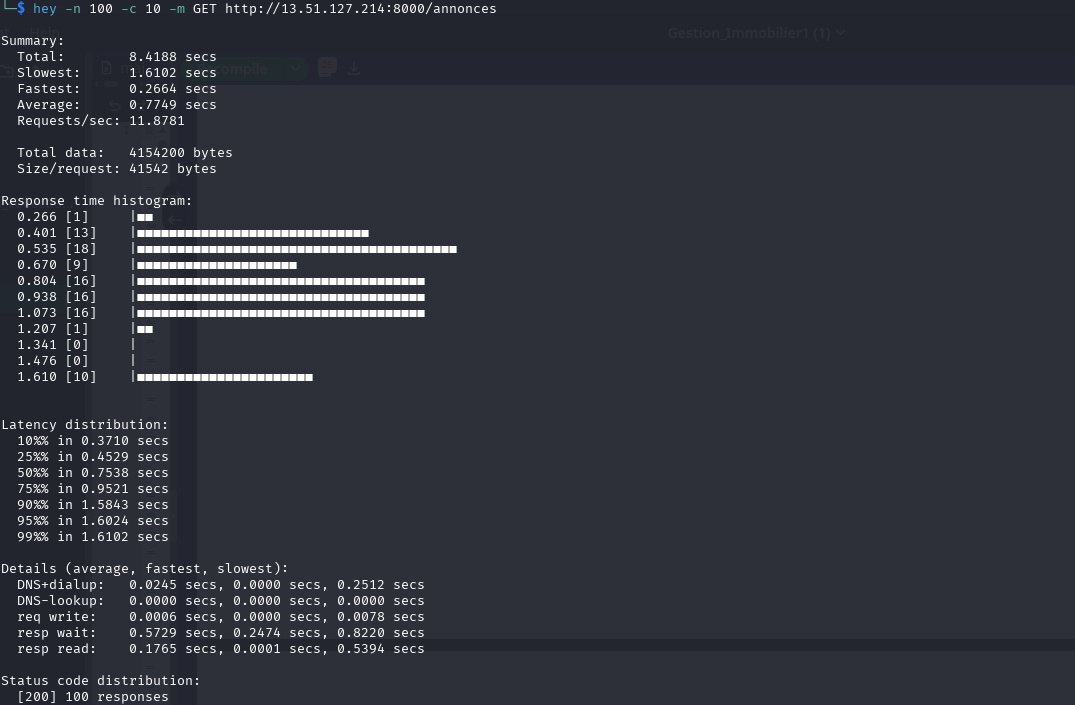
\includegraphics[width=\textwidth]{hey_results}
    \caption{Test de charge \texttt{hey} : 100 requ\^etes sur l'endpoint \texttt{/annonces} du serveur de production}
    \label{fig:hey_load_test}
\end{figure}


% ===========================================================
\section{Auto-\'evaluation des comp\'etences}
% ===========================================================
Au terme de ce stage, il nous semble important de porter un regard r\'etroactif sur les comp\'etences d\'evelopp\'ees, tant sur le plan technique qu'humain. Cette auto-\'evaluation s'articule autour de deux volets : les savoir-faire techniques (\emph{Hard Skills}) et le comportement en \'equipe (\emph{Soft Skills}).

\subsection{Comp\'etences techniques acquises (\emph{Hard Skills})}
Le tableau~\ref{tab:hard_skills} r\'esume les savoir-faire techniques que nous avons d\'evelopp\'es durant ce stage :

\begin{table}[H]
    \centering
    \small
    \renewcommand{\arraystretch}{1.3}
    \arrayrulecolor{black}
    \begin{tabularx}{\textwidth}{|l|X|}
        \hline
        \rowcolor{headergray}
        \textbf{Domaine} & \textbf{Ce que nous savons faire concr\`etement} \\ \hline
        \textbf{Python et FastAPI} & Cr\'eer un serveur web rapide capable de g\'erer plusieurs t\^aches en m\^eme temps. \\ \hline
        \textbf{Web Scraping} & \'Ecrire des robots d'extraction de donn\'ees capables de s'adapter aux diff\'erentes structures HTML des sites sources. \\ \hline
        \textbf{PostgreSQL} & Concevoir une base de donn\'ees organis\'ee en couches, avec historique et protection contre les \'ecrasements. \\ \hline
        \textbf{Flutter} & D\'evelopper une application mobile compl\`ete avec carte interactive et connexion au serveur. \\ \hline
        \textbf{Docker} & Isoler nos environnements de d\'eveloppement pour \'eviter les probl\`emes de compatibilit\'e. \\ \hline
    \end{tabularx}
    \caption{Comp\'etences techniques acquises durant le stage}
    \label{tab:hard_skills}
\end{table}

\subsection{Comportement en \'equipe (\emph{Soft Skills})}

\begin{table}[H]
    \centering
    \small
    \renewcommand{\arraystretch}{1.3}
    \arrayrulecolor{black}
    \begin{tabularx}{\textwidth}{|l|X|}
        \hline
        \rowcolor{headergray}
        \textbf{Qualit\'e} & \textbf{Comment elle s'est manifest\'ee dans le projet} \\ \hline
        \textbf{Travail d'\'equipe} & Division claire des t\^aches entre les trois membres : un sur l'interface mobile, un sur les robots, un sur la base de donn\'ees. \\ \hline
        \textbf{R\'esolution de probl\`emes} & Face aux d\'efis techniques (lenteur de l'algorithme, h\'et\'erog\'en\'eit\'e des sites sources), nous avons appris \`a chercher des solutions par nous-m\^emes. \\ \hline
        \textbf{Adaptabilit\'e} & Apprentissage rapide de technologies que nous n'avions jamais utilis\'ees avant le stage (Docker, FastAPI). \\ \hline
    \end{tabularx}
    \caption{Comp\'etences comportementales d\'evelopp\'ees durant le stage}
    \label{tab:soft_skills}
\end{table}

% ===========================================================
\section{Avis sur le stage}
% ===========================================================
Pour conclure ce bilan, nous souhaitons donner notre avis personnel sur cette exp\'erience professionnelle. Le stage a-t-il r\'epondu \`a nos attentes ?

La r\'eponse est clairement \textbf{oui}. Nous sommes arriv\'es avec des connaissances principalement th\'eoriques issues des cours magistraux, et nous avons eu la chance de les appliquer sur un projet concret et techniquement formateur. Ce stage nous a donn\'e l'opportunit\'e de participer \`a la conception d'un syst\`eme complet, de la base de donn\'ees jusqu'\`a l'application mobile, en passant par un algorithme de d\'eduplication. L'\'equipe de SSH nous a accord\'e une autonomie appr\'eci\'ee tout en restant disponible pour nous guider quand c'\'etait n\'ecessaire.

Si nous devions mentionner un point \`a am\'eliorer, ce serait la dur\'ee du stage. Le temps imparti ne nous a pas permis d'int\'egrer toutes les sources souhait\'ees (par exemple les groupes Facebook ou WhatsApp), ni d'optimiser pleinement les temps de r\'eponse de l'API. Malgr\'e cela, le prototype livr\'e est fonctionnel et test\'e, et constitue une base solide pour des it\'erations futures.

Cette exp\'erience nous a confirm\'e que le d\'eveloppement logiciel appliqu\'e aux probl\`emes concrets de notre soci\'et\'e est la voie dans laquelle nous souhaitons continuer \`a avancer.

\paragraph*{Conclusion du chapitre}
Ce chapitre a pr\'esent\'e les r\'esultats mesurables de notre travail au moment de la r\'edaction, nos apprentissages techniques et humains, ainsi que notre appr\'eciation du stage. Les donn\'ees collect\'ees montrent que CentralImmo, bien qu'encore limit\'e en couverture, r\'epond aux besoins identifi\'es et constitue une base que les it\'erations futures pourront enrichir. La conclusion g\'en\'erale qui suit r\'esumera l'ensemble du m\'emoire.

% ═══════════════════════════════════════════════════════════════
%  CONCLUSION GÉNÉRALE
% ═══════════════════════════════════════════════════════════════

\chapter*{Conclusion Générale}
\addcontentsline{toc}{chapter}{Conclusion Générale}

Ce stage avait pour objectif de concevoir et développer CentralImmo, une plateforme d'agrégation et de déduplication d'annonces immobilières pour le marché camerounais. Au terme de ce travail, plusieurs des objectifs fixés en introduction ont été atteints. Le pipeline de collecte fonctionne sur trois sources dédiées (Mapiole, Kasastay et Ny\`e Ta Piole) et a permis d'agréger 265 annonces au moment de la r\'edaction. L'algorithme de d\'eduplication DCS a identifi\'e environ 14\,\% de doublons parmi ces annonces, tous intra-source \`a ce stade. L'API REST FastAPI est op\'erationnelle ; un test de charge de 100 requ\^etes a atteint un taux de r\'eussite de 100\,\%, avec un temps de r\'eponse moyen d'environ 0{,}77 seconde sur l'endpoint principal. Enfin, une application mobile Flutter a \'et\'e livr\'ee et est fonctionnelle, bien que certaines optimisations restent n\'ecessaires.

La solution pr\'esente toutefois des limites qu'il convient de reconna\^itre. L'objectif initial de couvrir au moins trois sources a \'et\'e atteint, mais la troisi\`eme source (Ny\`e Ta Piole) n'a \'et\'e int\'egr\'ee qu'apr\`es la fin officielle du stage, le 16 juillet 2026, dans le cadre du prolongement du projet ; l'algorithme de d\'eduplication n'a pas encore pu \^etre valid\'e sur un volume important de doublons inter-sources. Le temps de r\'eponse de l'endpoint principal se situe au-dessus de l'objectif de 500\,ms fix\'e initialement, principalement en raison de l'absence de pagination. La couverture de tests automatis\'es reste partielle, limit\'ee aux endpoints API sans tests unitaires sur les modules de collecte et de d\'eduplication. Enfin, le seuil de fusion du DCS a \'et\'e fix\'e empiriquement, sans apprentissage supervis\'e sur un corpus \'etiquet\'e.

Les perspectives sont claires : étendre la collecte à de nouvelles plateformes et aux réseaux sociaux informels (Facebook, WhatsApp), mettre en place une pagination côté serveur pour améliorer les temps de réponse, calibrer le seuil DCS par apprentissage supervisé sur un corpus étiqueté, et constituer une suite de tests automatisés complète.

Ce stage confirme notre projet professionnel. La transformation de données brutes en information structurée, l'immersion en méthode agile chez SSH et notre contribution, encore modeste, à la centralisation de l'information immobilière camerounaise ont renforcé notre engagement dans la voie du développement logiciel appliqué au contexte local, et notre souhait de continuer dans cette direction après l'obtention de notre licence.


% ─────────────────────────────────────────────────────────────
%  ANNEXES & BIBLIOGRAPHIE
% ─────────────────────────────────────────────────────────────
% ═══════════════════════════════════════════════════════════════
%  ANNEXE A — Captures d'écran de l'application
% ═══════════════════════════════════════════════════════════════

\chapter*{Annexe A --- Captures d'écran de l'application}
\addcontentsline{toc}{chapter}{Annexe A --- Captures d'écran de l'application}
\label{annexe:screens}

\section*{A.1 --- Interface mobile}

\begin{figure}[H]
    \centering
    \begin{minipage}[t]{0.45\textwidth}
        \centering
        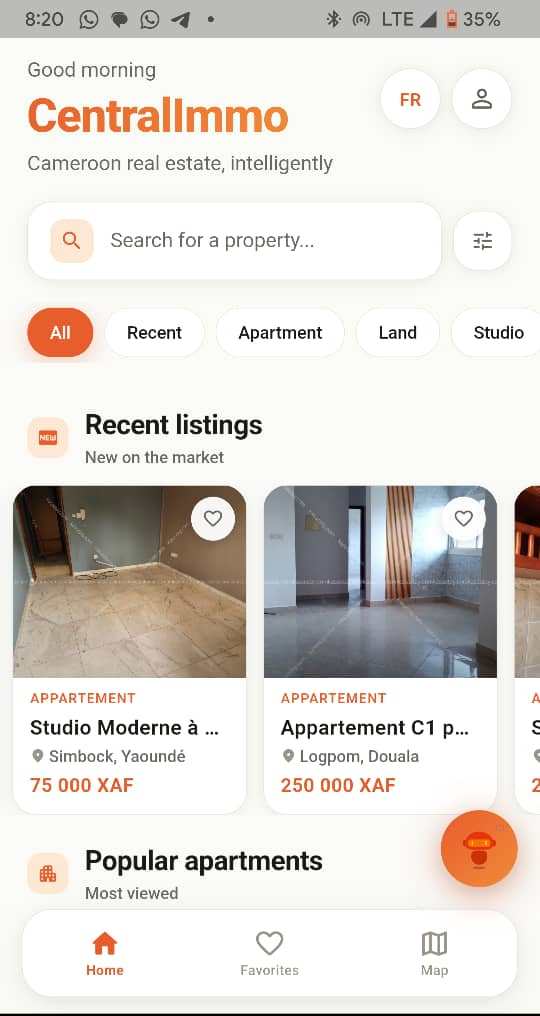
\includegraphics[width=\linewidth]{HomeMobile.jpeg}
        \caption*{\'Ecran d'accueil mobile --- liste des annonces}
    \end{minipage}
    \hfill
    \begin{minipage}[t]{0.45\textwidth}
        \centering
        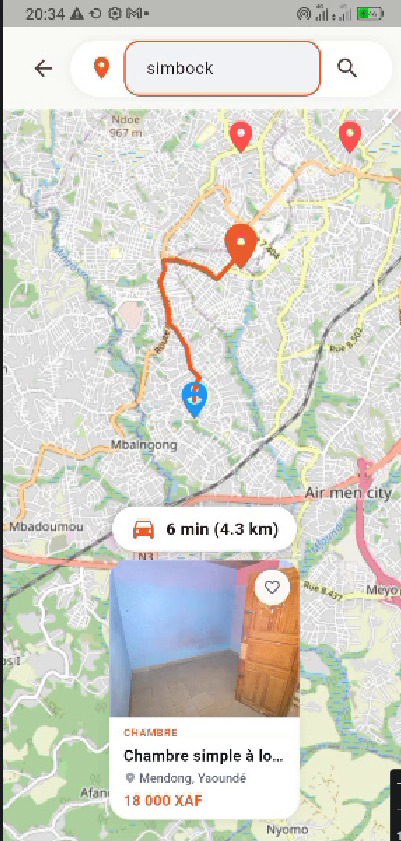
\includegraphics[width=\linewidth]{MobileMapsRecherche.jpeg}
        \caption*{Recherche par itin\'eraire mobile}
    \end{minipage}
\end{figure}

\begin{figure}[H]
    \centering
    \begin{minipage}[t]{0.45\textwidth}
        \centering
        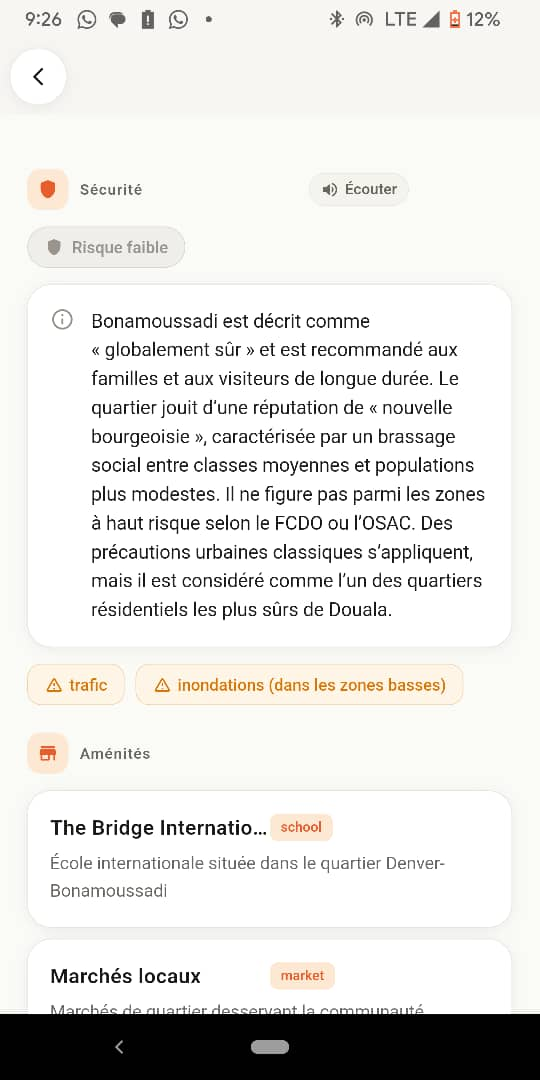
\includegraphics[width=\linewidth]{MobileDetails.jpeg}
        \caption*{D\'etail d'un bien --- intelligence de quartier mobile}
    \end{minipage}
\end{figure}

\section*{A.2 --- Interface web}

\begin{figure}[H]
    \centering
    \begin{minipage}[t]{0.48\textwidth}
        \centering
        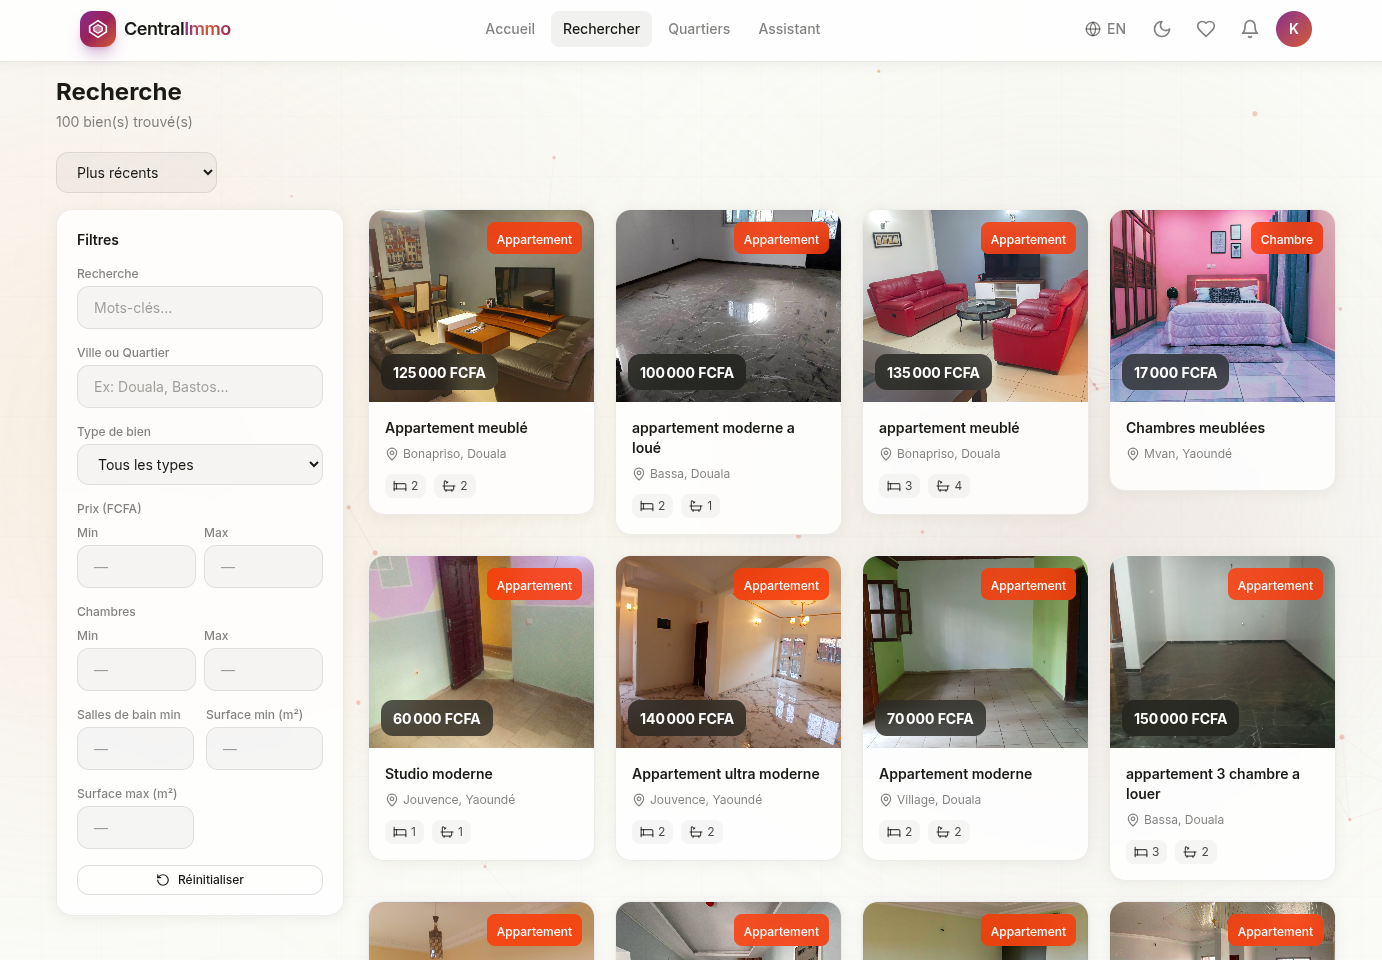
\includegraphics[width=\linewidth]{WebResearch.png}
        \caption*{Page de recherche web --- filtres et annonces}
    \end{minipage}
    \hfill
    \begin{minipage}[t]{0.48\textwidth}
        \centering
        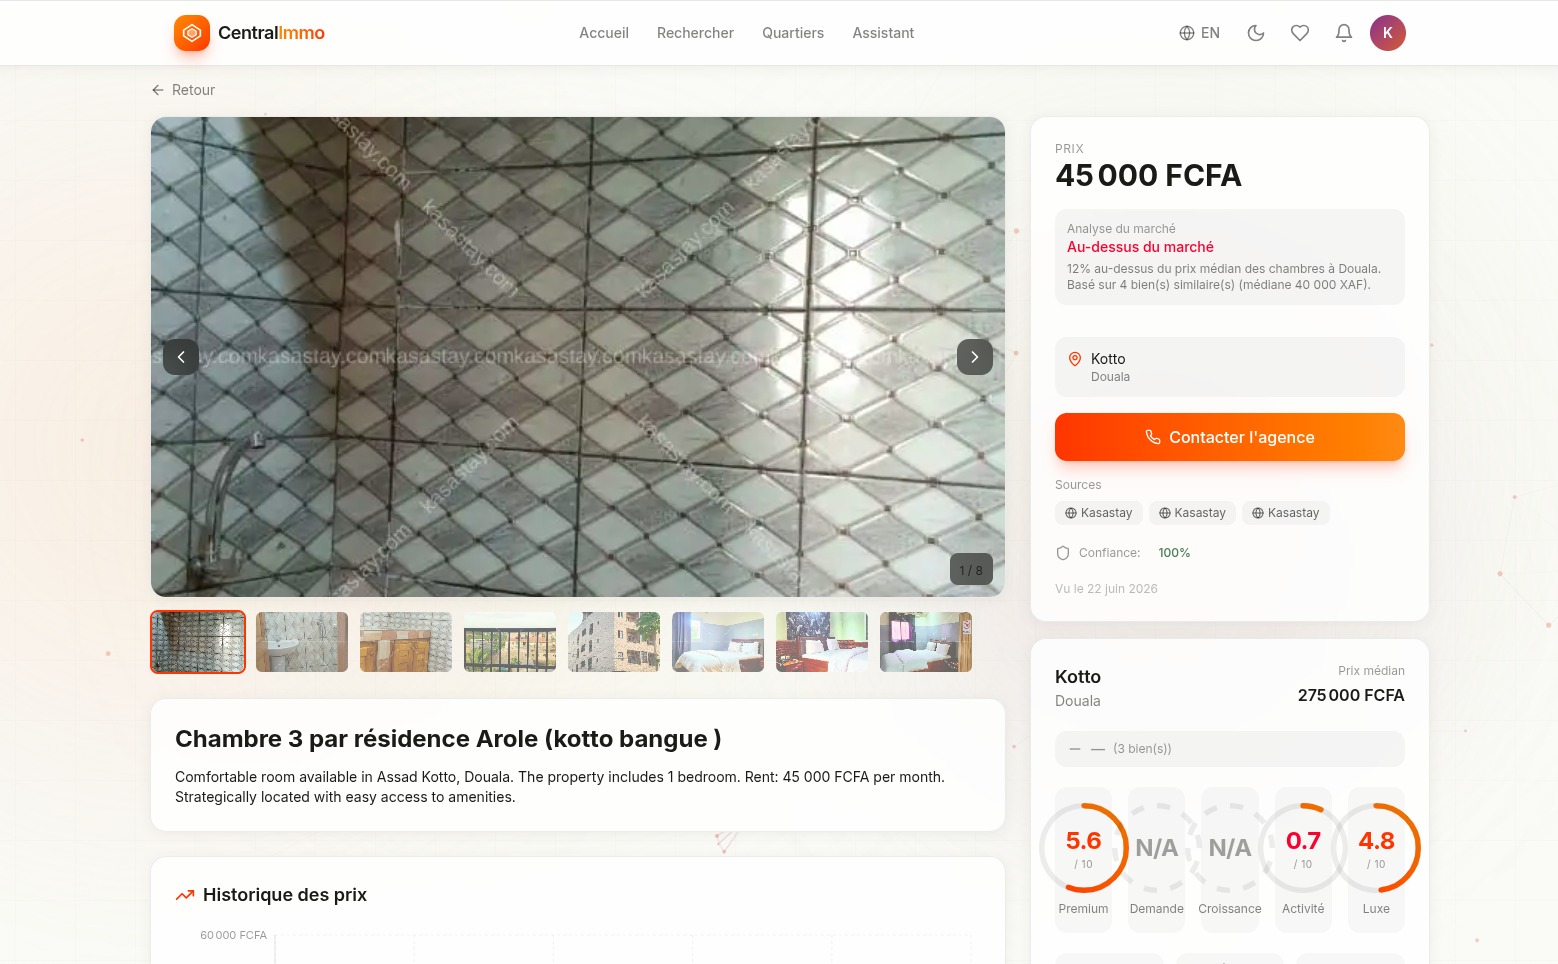
\includegraphics[width=\linewidth]{WebDetails.png}
        \caption*{Page de d\'etail d'un bien --- vue web}
    \end{minipage}
\end{figure}

% ═══════════════════════════════════════════════════════════════
%  ANNEXE B — Diagrammes de séquence
% ═══════════════════════════════════════════════════════════════

\chapter*{Annexe B --- Diagrammes de s\'equence}
\addcontentsline{toc}{chapter}{Annexe B --- Diagrammes de s\'equence}
\label{annexe:sequences}

\begin{figure}[H]
    \centering
    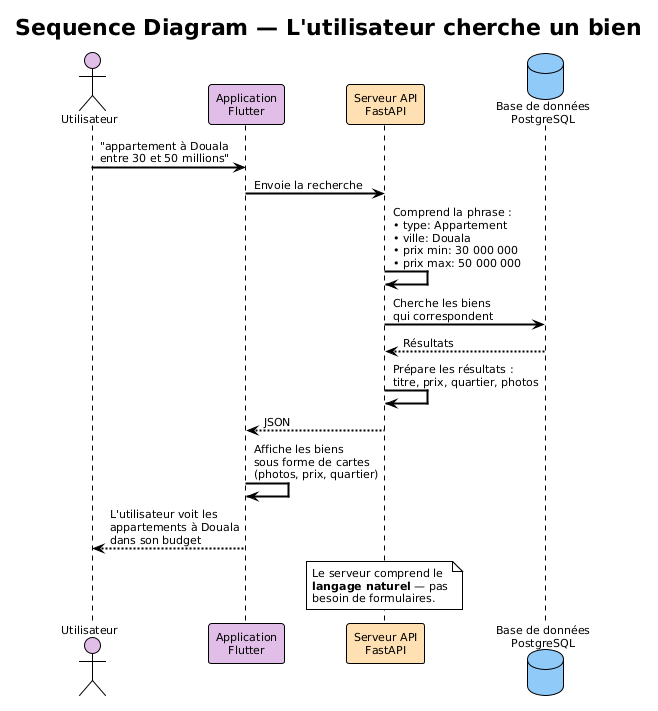
\includegraphics[width=0.9\textwidth]{Sequence Recherche.png}
    \caption{S\'equence de recherche d'un bien}
    \label{fig:annexe_sequence_recherche}
\end{figure}

\begin{figure}[H]
    \centering
    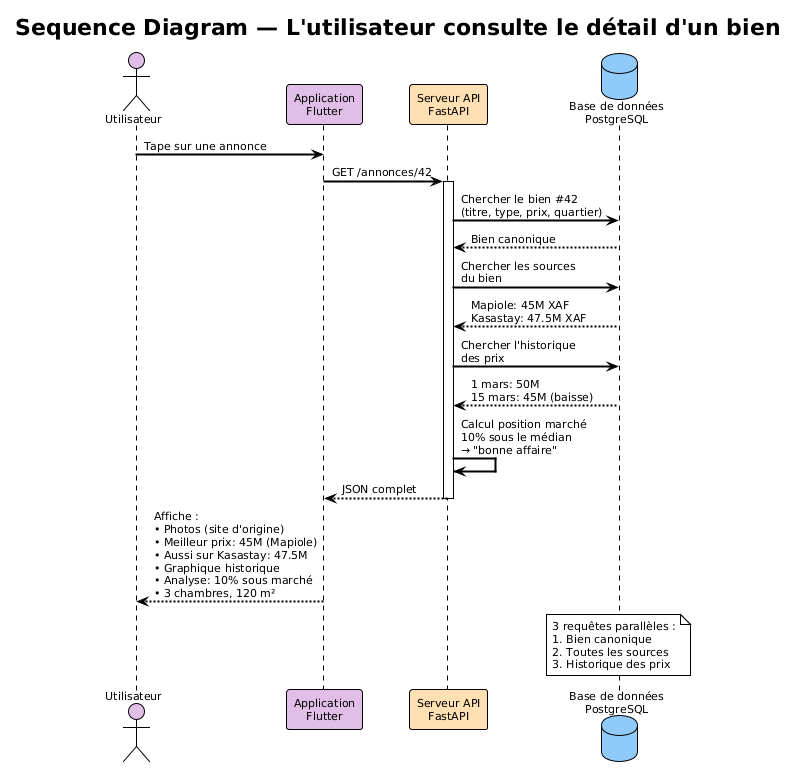
\includegraphics[width=0.9\textwidth]{Sequence Detail Bien.png}
    \caption{S\'equence de consultation du d\'etail d'un bien}
    \label{fig:annexe_sequence_detail}
\end{figure}

% ═══════════════════════════════════════════════════════════════
%  ANNEXE C — Endpoints de l'API REST
% ═══════════════════════════════════════════════════════════════

\chapter*{Annexe C --- Endpoints de l'API REST}
\addcontentsline{toc}{chapter}{Annexe C --- Endpoints de l'API REST}
\label{annexe:api}

L'API REST expos\'ee par le back-end FastAPI est organis\'ee en routeurs th\'ematiques. Le tableau ci-dessous recense les principaux endpoints consomm\'es par l'application mobile et web.

\begin{table}[H]
    \centering
    \footnotesize
    \renewcommand{\arraystretch}{1.25}
    \begin{tabularx}{\textwidth}{|l|l|X|}
        \hline
        \rowcolor{headergray}
        \textbf{M\'ethode} & \textbf{Chemin} & \textbf{Description} \\ \hline
        GET  & \texttt{/health} & Sonde de vie du serveur (statut DB, scheduler). \\ \hline
        GET  & \texttt{/annonces} & Liste pagin\'ee des fiches canoniques (filtrable par type, prix, surface, chambres). \\ \hline
        GET  & \texttt{/annonces/nearby} & Fiches canoniques proches d'un point (lat, lng, rayon). \\ \hline
        GET  & \texttt{/annonces/\{id\}} & D\'etail consolid\'e d'une fiche canonique (sources li\'ees, prix compar\'es). \\ \hline
        GET  & \texttt{/annonces/\{id\}/history} & Historique des \'ev\'enements (prix, disponibilit\'e) d'une annonce. \\ \hline
        GET  & \texttt{/annonces/\{id\}/similar} & Fiches canoniques similaires (m\^eme type, m\^eme quartier). \\ \hline
        GET  & \texttt{/annonces/\{id\}/analyse} & Analyse de positionnement de prix vs quartiers comparables. \\ \hline
        GET  & \texttt{/search} & Recherche en langage naturel (parse la requ\^ete c\^ot\'e serveur). \\ \hline
        GET  & \texttt{/search/ai} & Variante assist\'ee par IA de la recherche naturelle. \\ \hline
        POST & \texttt{/chat} & Assistant conversationnel (questions sur le march\'e). \\ \hline
        GET  & \texttt{/neighborhoods} & Liste des localisations connues (villes + quartiers). \\ \hline
        GET  & \texttt{/neighborhoods/\{slug\}} & Indicateurs d'un quartier (prix m\'edian, dur\'ee de publication, score d'activit\'e). \\ \hline
        GET  & \texttt{/neighborhoods/city/\{city\}} & Indicateurs agr\'eg\'es par ville. \\ \hline
        GET  & \texttt{/neighborhoods/trending/list} & Quartiers en croissance (tendance 90 jours). \\ \hline
        GET  & \texttt{/profiles/cities} & Profils de ville complets (price\_tier, growth, demand). \\ \hline
        GET  & \texttt{/profiles/neighborhoods/by-location/\{id\}} & Profil complet d'un quartier. \\ \hline
        GET  & \texttt{/admin/review/pending} & Annonces en attente de validation humaine (adaptateur universel). \\ \hline
        POST & \texttt{/admin/review/\{raw\_id\}} & Approuver ou refuser une annonce en attente. \\ \hline
        GET  & \texttt{/admin/sources} & Liste des sources configur\'ees. \\ \hline
        POST & \texttt{/admin/sources} & Ajouter une nouvelle source (slug, URL, type d'adaptateur). \\ \hline
        POST & \texttt{/admin/sources/\{slug\}/crawl} & D\'eclencher manuellement une collecte pour une source. \\ \hline
        POST & \texttt{/admin/analytics/recompute} & Recalculer les scores de quartiers \`a la demande. \\ \hline
        GET  & \texttt{/admin/jobs} & \'Etat des t\^aches programm\'ees (APScheduler). \\ \hline
        POST & \texttt{/payments/upgrade} & Souscription \`a un plan payant (int\'egration Mobile Money). \\ \hline
        GET  & \texttt{/payments/\{ref\}/status} & Statut d'une transaction. \\ \hline
    \end{tabularx}
    \caption{Principaux endpoints de l'API CentralImmo}
    \label{tab:api_endpoints}
\end{table}

% ═══════════════════════════════════════════════════════════════
%  ANNEXE D — Extraits du code source
% ═══════════════════════════════════════════════════════════════

\chapter*{Annexe D --- Extraits du code source}
\addcontentsline{toc}{chapter}{Annexe D --- Extraits du code source}
\label{annexe:code}

\section*{D.1 --- Algorithme de d\'eduplication (DCS)}

Calcul du Duplicate Confidence Score entre une annonce brute et une fiche canonique (\texttt{core/matcher.py}).

\begin{lstlisting}[language=Python, caption={Calcul du DCS --- \texttt{compute\_dcs}}, label={lst:dcs}]
def compute_dcs(draft, canonical, draft_location_id=None):
    f = MatchFactors(
        title_sim=_title_sim(draft.title_raw, canonical.title_canonical),
        price_proximity=_price_proximity(
            draft.price_parsed, canonical.current_best_price),
        type_match=1.0 if (draft.property_type_raw or "").lower()
            == (canonical.property_type or "").lower() else 0.0,
        surface_match=_surface_match(draft.area_sqm, canonical.area_sqm),
        bedrooms_match=_exact_or_neutral(draft.bedrooms, canonical.bedrooms),
        location_sim=_location_sim(draft_location_id,
            canonical.location_id, draft.location_raw, None),
        image_overlap=_image_overlap(draft.images_raw or [], []),
    )
    dcs = (
        0.30 * f.title_sim
        + 0.20 * f.price_proximity
        + 0.15 * f.type_match
        + 0.15 * f.surface_match
        + 0.10 * f.bedrooms_match
        + 0.05 * f.location_sim
        + 0.05 * f.image_overlap
    )
    return dcs, f
\end{lstlisting}

\section*{D.2 --- Idempotence du pipeline d'ingest}

\`A chaque collecte, le robot calcule un \texttt{url\_hash} (sha256 de l'URL normalis\'ee). S'il existe d\'ej\`a, l'annonce n'est pas r\'eins\'er\'ee : on met \`a jour sa date de collecte et on enregistre un \'ev\'enement d'historique uniquement si le prix ou la disponibilit\'e ont chang\'e (\texttt{core/ingest.py}).

\begin{lstlisting}[language=Python, caption={Boucle d'ingest idempotente}, label={lst:ingest}]
def ingest(db, drafts, source_id, crawl_session_id, adapter_kind="dedicated"):
    for draft in drafts:
        url_hash = hashlib.sha256(
            normalize_url(draft.url_source).encode("utf-8")).hexdigest()
        existing = db.query(RawListing).filter(
            RawListing.url_hash == url_hash).first()
        if existing:
            # RE-CRAWL: ne pas re-inserer, juste comparer a l'historique
            existing.crawl_session_id = crawl_session_id
            existing.crawled_at = datetime.now(timezone.utc)
            if existing.canonical_property_id:
                append_history_if_changed(db, existing.id,
                    existing.canonical_property_id, draft.price_parsed,
                    "available", crawl_session_id)
            continue
        # NOUVELLE annonce : resolution de localisation + match canonique
        location_id = resolve_location(db, draft.location_raw)
        match_result = find_canonical_match(db, draft, location_id)
        # ... insertion du RawListing + lien/creation du CanonicalProperty ...
\end{lstlisting}

\section*{D.3 --- Normalisation d'une annonce Ny\`e Ta Piole}

Le m\'ecanisme de conversion d'un JSON brut de l'API Ny\`e Ta Piole vers le format unifi\'e \texttt{RawListingDraft} (\texttt{scrapers/nyetapiole.py}). Les champs \texttt{surface}, \texttt{bedrooms} et coordonn\'ees \`a \texttt{0} sont convertis en \texttt{None} pour \'eviter de polluer la fiche canonique avec des donn\'ees absentes.

\begin{lstlisting}[language=Python, caption={Normalisation Ny\`e Ta Piole --- extrait}, label={lst:nyetapiole}]
def normalize_data(self, raw):
    slug = raw.get("slug")
    title = raw.get("title", "").strip()
    if not slug or not title:
        return None
    price = raw.get("price")
    price_parsed = int(price) if isinstance(price, (int, float)) and price > 0 else None
    district = raw.get("district") or {}
    city_name = (district.get("city") or {}).get("name", "")
    district_name = district.get("name", "")
    location_raw = f"{district_name}, {city_name}" if district_name and city_name else (city_name or district_name)
    lat = raw.get("latitude")
    lng = raw.get("longitude")
    latitude = float(lat) if isinstance(lat, (int, float)) and lat != 0 else None
    longitude = float(lng) if isinstance(lng, (int, float)) and lng != 0 else None
    bedrooms = raw.get("bedrooms")
    bedrooms = bedrooms if isinstance(bedrooms, int) and bedrooms > 0 else None
    surface = raw.get("surface")
    area_sqm = float(surface) if isinstance(surface, (int, float)) and surface > 0 else None
    return RawListingDraft(
        url_source=f"https://nyetapiole.com/property/{slug}",
        title_raw=title, price_parsed=price_parsed, currency="XAF",
        location_raw=location_raw, bedrooms=bedrooms, area_sqm=area_sqm,
        latitude=latitude, longitude=longitude, confidence=1.0,
    )
\end{lstlisting}
% ═══════════════════════════════════════════════════════════════
%  RÉFÉRENCES BIBLIOGRAPHIQUES
% ═══════════════════════════════════════════════════════════════

\chapter*{Références Bibliographiques}
\addcontentsline{toc}{chapter}{Références Bibliographiques}

Cette section répertorie les documents, articles, sites web et guides de l'industrie exploités tout au long de la conception et du développement de la plateforme CentralImmo. Les références sont citées dans le texte selon la norme IEEE (numérotation entre crochets).

\bigskip

\begin{enumerate}[label={[\arabic*]}, leftmargin=1.2cm, labelsep=0.3cm, itemsep=0.8em]

    \item \label{ref:ndah} \textbf{Ndah Gilgar}, «~The problem with real estate data in Cameroon --- and why I decided to build StratAxis~», \textit{LinkedIn Post}, mars 2026. [En ligne]. Disponible~: \url{https://www.linkedin.com/posts/strataxis_the-problem-with-real-estate-data-in-cameroon-activity-7433933407119794176-86OI}

    \item \label{ref:strataxis} \textbf{StratAxis Cameroon}, «~Why Cameroon Needs a Real Estate Intelligence Layer~», \textit{LinkedIn Post}, mars 2026. [En ligne]. Disponible~: \url{https://www.linkedin.com/posts/strataxis_why-cameroon-needs-a-real-estate-intelligence-activity-7433933915427450880-hSDu}

    \item \label{ref:mapiole_app} \textbf{Mapiole S.A.S.}, \textit{Mapiole --- Acheter, Vendre, Louer \& Construire au Cameroun}, Page officielle, 2026. [En ligne]. Disponible~: \url{https://www.mapiole.com}

    \item \label{ref:ownkey_portals} \textbf{Ownkey}, «~Best Real Estate Portals in Africa 2026: The Complete Country-by-Country Guide~», \textit{Ownkey Blog}, avril 2026. [En ligne]. Disponible~: \url{https://ownkey.com/blog/best-real-estate-portals-africa}

    \item \label{ref:ownkey_nigeria} \textbf{Ownkey}, «~Nigeria's Biggest Property Portal: Does `Most Listings' Actually Mean Best for Buyers? The Truth About Ghost Listings~», \textit{Ownkey Blog --- Nigeria}, juin 2026. [En ligne]. Disponible~: \url{https://ownkey.com/ng/blog}

    \item \label{ref:knf} \textbf{KnF Properties SARL}, «~À propos de nous --- Vérification et protection foncière au Cameroun~», \textit{KnF Properties}, 2025. [En ligne]. Disponible~: \url{https://knfproperties.com/fr/about-us}

    \item \label{ref:africanvestor} \textbf{The Africanvestor}, «~Cameroon Real Estate Market Analysis (2026)~», \textit{The Africanvestor Blog}, 2026. [En ligne]. Disponible~: \url{https://theafricanvestor.com/blogs/news/cameroon-real-estate-market}

    \item \label{ref:datareportal} \textbf{We Are Social / DataReportal}, \textit{Digital 2025: Cameroon}, Rapport sur les indicateurs mobiles et internet, 2025. [En ligne]. Disponible~: \url{https://datareportal.com/reports/digital-2025-cameroon}

    \item \label{ref:fastapi} \textbf{FastAPI}, \textit{FastAPI --- Python framework, high performance}, Documentation officielle, 2026. [En ligne]. Disponible~: \url{https://fastapi.tiangolo.com}

    \item \label{ref:flutter} \textbf{Flutter}, \textit{Flutter --- Build for any screen}, Site officiel du framework, 2026. [En ligne]. Disponible~: \url{https://flutter.dev}

    \item \label{ref:postgres_es} \textbf{Neon}, «~Comparing Native Postgres, ElasticSearch, and pg\_search for Full-Text Search~», \textit{Neon Blog}, juin 2025. [En ligne]. Disponible~: \url{https://neon.com/blog/postgres-full-text-search-vs-elasticsearch}

    \item \label{ref:docker} \textbf{Nick Janetakis}, «~Best Practices Around Production Ready Web Apps with Docker Compose~», \textit{Blog Post}, mai 2021. [En ligne]. Disponible~: \url{https://nickjanetakis.com/blog/best-practices-around-production-ready-web-apps-with-docker-compose}

    \item \label{ref:beautifulsoup} \textbf{BeautifulSoup}, \textit{Beautiful Soup Documentation}, crummy.com, 2024. [En ligne]. Disponible~: \url{https://www.crummy.com/software/BeautifulSoup/}

    \item \label{ref:rapidfuzz} \textbf{RapidFuzz}, \textit{RapidFuzz --- fast string matching}, Documentation officielle, 2024. [En ligne]. Disponible~: \url{https://rapidfuzz.github.io/RapidFuzz/}

    \item \label{ref:apscheduler} \textbf{APScheduler}, \textit{Advanced Python Scheduler}, Documentation officielle, 2024. [En ligne]. Disponible~: \url{https://apscheduler.readthedocs.io/}

    \item \label{ref:postgresql} \textbf{PostgreSQL}, \textit{PostgreSQL 16 Documentation}, The PostgreSQL Global Development Group, 2024. [En ligne]. Disponible~: \url{https://www.postgresql.org/docs/}

    \item \label{ref:beac} \textbf{Banque des États de l'Afrique Centrale (BEAC)}, \textit{Rapport sur la politique monétaire et l'évolution économique en zone CEMAC}, mars 2023. [En ligne]. Disponible~: \url{https://www.beac.int/publications/rapport-de-politique-monetaire/}

    \item \label{ref:ins} \textbf{Institut National de la Statistique (INS)}, \textit{EESI3 Phase 2 : Enquête sur le Secteur Informel au Cameroun --- Rapport principal}, novembre 2023. [En ligne]. Disponible~: \url{https://ins-cameroun.cm/statistique/eesi3-phase-2-enquete-sur-le-secteur-informel-rapport-principal/}

    \item \label{ref:keurimmo} \textbf{KEUR-IMMO}, \textit{KEUR-IMMO --- 1\textsuperscript{er} site d'annonces immobilières en Afrique francophone}, Page officielle, 2026. [En ligne]. Disponible~: \url{https://keur-immo.com/en/cameroon/}

    \item \label{ref:puol} \textbf{PUOL}, \textit{PUOL --- Application de mise en relation propriétaires/locataires au Cameroun}, Page officielle LinkedIn, 2026. [En ligne]. Disponible~: \url{https://www.linkedin.com/company/puol-app}

    \item \label{ref:nyetapiole} \textbf{Nyè Ta Piole}, \textit{Nyè Ta Piole --- La première proptech camerounaise qui connecte propriétaires et locataires}, Site officiel, 2026. [En ligne]. Disponible~: \url{https://nyetapiole.com}

\end{enumerate}

\end{document}